\documentclass[../main.tex]{subfiles}
\graphicspath{{\subfix{../figures/}}}

\begin{document}

\chapter{{DiffFracSeq: A Bayesian Model for the Detection of Differential Fractionation of Sequencing Data}}

\section{Introduction}

\begin{figure}

{\centering 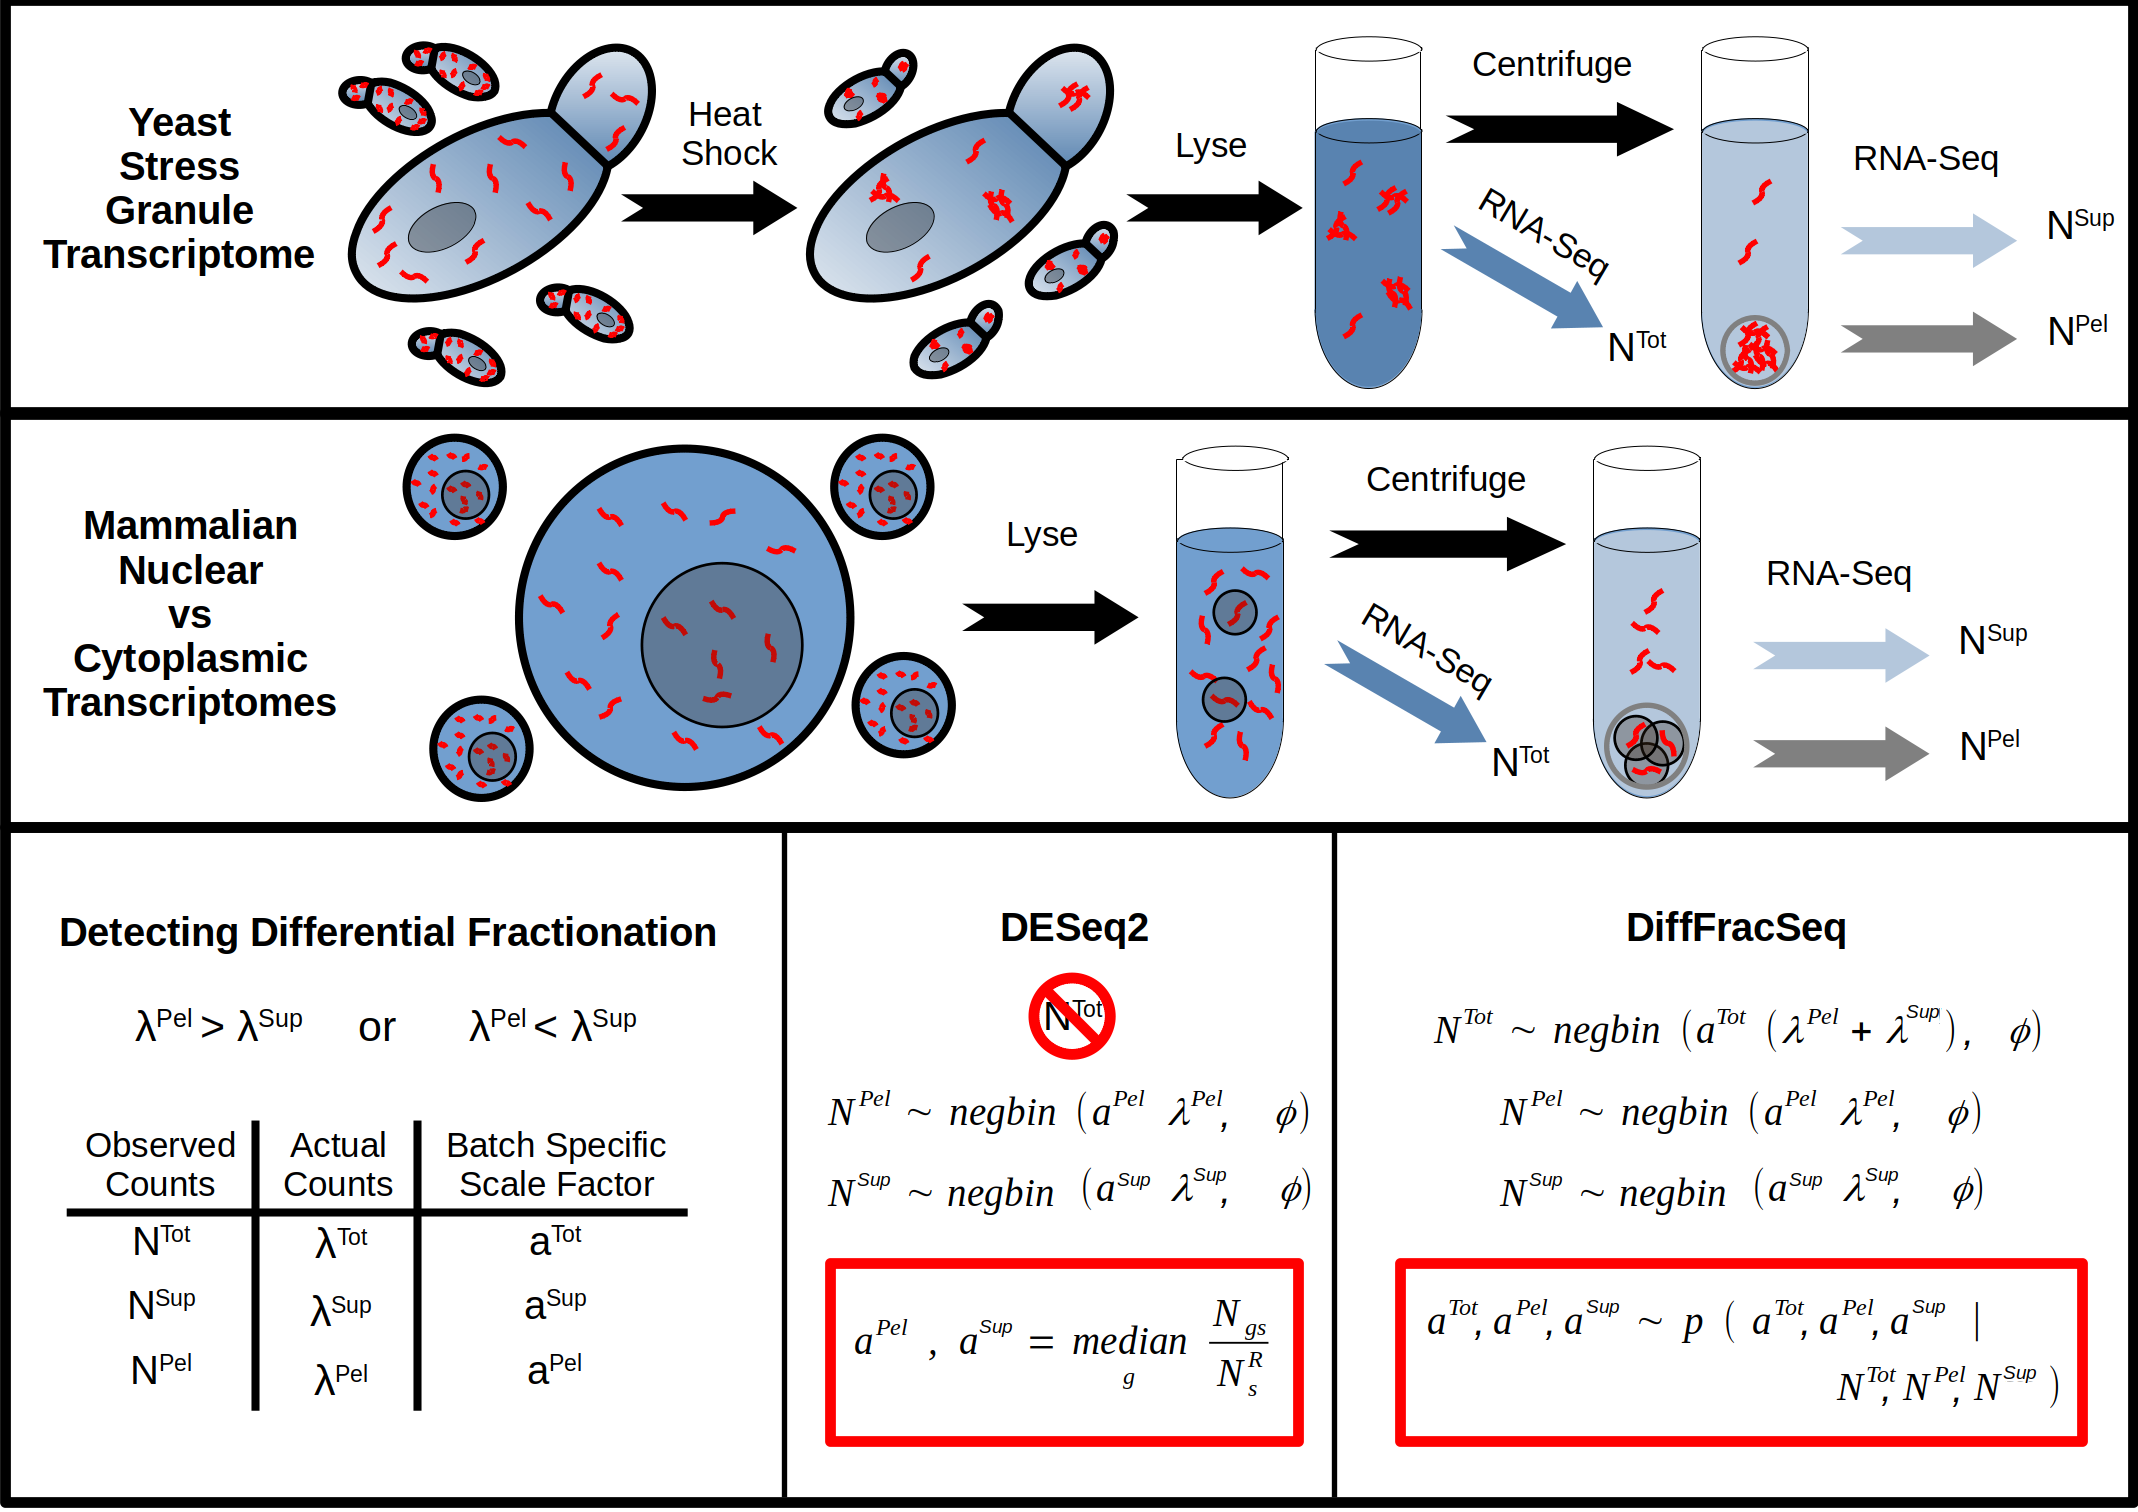
\includegraphics[width=1\linewidth]{figures/diffFracSeq_diagram.png} 

}

\caption[DiffFracSeq chapter summary.]{\textbf{Summary of two different fractionation experiments and comparison of detecting differential fractionation with DESeq2 vs DiffFracSeq.} The top panel summarises a fractionation experiment by Iserman \textit{et al} that investigates the transcriptome of stress granules formed by yeast cells in response to heat stress \parencite{Iserman2020}. The middle panel summarises a fractionation experiment by the ENCODE consortium to compare the nuclear and cytoplasmic transcriptomes in lymphoblastoid cells \parencite{Dunham2012}. Both panels highlight the stages at which RNA-Seq samples are taken: one before fractionation, $N^{Tot}$, and two after fractionation, $N^{Sup}$ and $N^{Pel}$. The bottom panel outlines the task of detecting differential fractionation using noisy RNA-Seq transcript counts. The RNA-Seq count models behind DESeq2 and DiffFracSeq are also summarised with key differences highlighted in red.}. \label{fig:diffFracSeq-diagram}
\end{figure}

Localisation of RNA populations to specific sub-cellular compartments is used to regulate gene expression across the tree of life \parencite{Das2021}.
A ubiquitous example is the distinct populations of RNA found to be localised to the nucleus or the cytoplasm. 
Most mRNA transcripts are localised in the cytoplasm in order to be translated \parencite{Kohler2007}.
Many non-coding RNA (ncRNA) transcripts, such as those that facilitate splicing, are localised to the nucleus \parencite{Will2011}. 
In plant and animal cells, microRNA (miRNA), long non-coding RNA (lncRNA) and small interfering RNA (siRNA) contribute to gene expression regulation through splicing, degradation or translation pathways specific either to the nucleus or cytoplasm \parencite{Hombach2016}.
Localisation also aids in the transportation of secretory proteins as their mRNA transcripts are co-translationally translocated to the endoplasmic reticulum \parencite{Jan2014}.

Localisation can enable rapid changes in gene expression in response to stress or facilitate precise changes at highly sensitive stages of cell cycles.
In response to stimuli, such as heat stress, surplus mRNA transcripts can be collected into stress granules where translation may be suppressed \parencite{Anderson2009}. 
Previous studies have shown that between 10\%-15\% of mRNA transcripts are localised to granules when exposed to stress \parencite{VanTreeck2018,Khong2017}.
The mRNA transcripts enriched in stress granules are characterised by poor translatability and long coding region/3' UTR length \parencite{Khong2017}.
Granules of ribonucleoproteins, such as processing bodies (P-bodies), also facilitate the tight regulatory control of translation without degrading mRNA \parencite{Buchan2014}.
In \textit{C. elegans}, oogenesis includes the release of nuclear-bound P-bodies into the cytoplasm during prophase I \parencite{Voronina2011}.
Meanwhile, mutations that affect the formation of ribonucleoprotein granules are associated with several human diseases \parencite{Mackenzie2017}. 

Several RNA-Seq assays have been developed to investigate RNA localisation by isolating and comparing RNA populations in different sub-cellular compartments.
Fractions of mRNA from organelles of different densities can be separated by centrifuging cell lysate. 
Centrifuging using a sucrose gradient or by repeatedly centrifuging the supernatant under increasing speeds can separate a sample into multiple fractions \parencite{Iserman2020, Dunham2012, Hu2017}.
Experiments can also include an immunopurification step after centrifugation to further purify samples with compartments of interest \parencite{Khong2017}.
Alternatively, fractions of freely floating vs protein-bound mRNA can be separated by orthogonal organic phase separation \parencite{Queiroz2019}. 

Despite the development of multiple fractionation-based RNA-Seq assays, there are no statistical methods designed to detect differential fractionation.
Previous studies to determine changes in transcript abundance across different fractions have had to use statistical software developed to determine differential expression across conditions. 
DESeq \parencite{Anders2010}, edgeR \parencite{Robinson2010} and Cuffdiff \parencite{Trapnell2010} have been used in attempts to determine differential fractionation in yeast and human data sets \parencite{Khong2017, Matheny2019, VanTreeck2018, Hubstenberger2017}. 
Unfortunately, these methods address sequencing bias by assuming only a subset of genes will experience biologically significant differences across conditions. 
Under this assumption, the change in the average gene is not biological, but must be down to sequencing bias; predominately the batch-specific library size.
Quantile normalisation techniques, such as the median of medians used by DESeq, attempt to find an average gene to normalise to across the conditions and reduce the sequencing bias \parencite{Anders2010}.
However, the assumption breaks down in cases where the majority of genes are expected to have different expressions across RNA-Seq samples. 
For example, in assays that extract RNA from different fractions, changes in abundance across the entire transcriptome may be expected.
These methods also estimate sequencing bias \textit{a priori} and any uncertainty in their values is not included in the tests for differential expression.


This work presents DiffFracSeq, a Bayesian statistical model specifically designed to detect differential fractionation.
The chapter outlines an alternative way of normalising RNA-Seq data sets from different fractions using the additional information that can be gathered when measuring subsets of a complete sample.
The normalising method uses the transcript counts of samples taken before fractionation to enable reliable inference of RNA-Seq batch-specific scale factors within the Bayesian model, rather than relying on \textit{a priori} estimations.
First, the model behind DiffFracSeq is introduced and its ability to model noisy RNA-Seq transcript counts is tested using a simulated data set. 
The simulated data set is also used to show the limitations of using quantile normalisation methods in experiments with global changes in the transcriptome by using DESeq2 to detect differential fractionation \parencite{Love2014}.
Then, DESeq2 and DiffFracSeq are applied to two experimental data sets, outlined in Figure \ref{fig:diffFracSeq-diagram}, and their ability to detect differential fractionation is compared.
DiffFracSeq is an open-source R software package that will enable even more sensitive comparisons of transcript localisation across conditions and cell types.

\section{Results}

\subsection{Bayesian hierarchical model}

The DiffFracSeq model reliably detects differential fractionation by: A) using RNA-Seq counts taken from a sample before fractionation as a quasi-replicate to provide additional information with which to normalise the counts taken from the fractionation samples, and B) including the determination of batch-specific scale factors within the Bayesian framework rather than depending on \textit{a priori} estimations.
The normalisation of the counts from different fractions can be aided by the counts from a pre-fractionation sample if the sum of transcripts counts from sub-fractions is assumed to equal the counts from the total body; i.e. $N^{Tot} = N^{A}+N^{B}$.
Summing the counts across all fractions accounts for the expected global changes in their transcriptomes, but any difference between this sum and a sample from the total body can be assumed to come from sequencing bias rather than biological effect.
Therefore, the sample taken before fractionation can be considered a quasi-replicate that enables information to be shared across fractions to account for the sequence bias.

The Bayesian model determines values for noiseless transcript counts $\lambda$, overdispersion parameters $\phi$, and batch-specific library scale factors $a$.
The noise of transcript counts from RNA-Seq data is modelled by a negative binomial with mean $\lambda$ and overdispersion parameter $\phi$, as RNA-Seq transcript counts are positive integers and overdispersion is often present \parencite{Robinson2007,Cameron1998}.
The DiffFracSeq model contains three negative binomial distributions: one for samples from the total body and one for each of the two sub-fractions Figure \ref{fig:DiffFracQuant-plate-diagram}.
The three negative binomial distributions each have an overdispersion parameter: $\phi^{Tot}$, $\phi^{A}$ and $\phi^{B}$, that is shared across genes and conditions.
Separate mean parameters for transcript counts are learnt for the sub-fraction negative binomials: $\lambda^A$ and $\lambda^B$, and their sum is used as the mean for the total negative binomial.
The $\lambda$ parameters are determined in log space to help the model fit the broad range of transcript count levels expected across an entire genome.
In addition to the mean transcript count parameter, each negative binomial has a total reads scale factor term: $a^{Tot}$, $a^{A}$, $a^{B}$, that is unique to the condition and replicate used.
The R package RStan is used to sample from the posterior distribution, the core stan code is available in Appendix C.

\begin{figure} [t!]
     \centering
     \begin{subfigure}[b]{0.4\textwidth}
     \centering
     \tikz{
        % Nodes
        \node[obs]                                   (N-t)   {$N^{Tot}_{gr}$}; %
        \node[obs, above=1 of N-t, xshift=-1.2cm]     (N-s)   {$N^{A}_{gr}$}; %
        \node[obs, right=1 of N-s, xshift=0.4cm]     (N-p)   {$N^{B}_{gr}$}; %
        \node[latent, above=1 of N-s]  (l-s)   {$\lambda^{A}_{g}$}; %
        \node[latent, above=1 of N-p] (l-p)   {$\lambda^{B}_{g}$}; %
        \node[latent, left=2 of N-t, xshift=-1cm] (p-t)     {$\phi^{Tot}$}; %
        \node[latent, above=1 of p-t] (p-s)     {$\phi^{A}$}; %
        \node[latent, right=1 of N-p, xshift=0.4cm] (p-p)     {$\phi^{B}$}; %
        \node[latent, below=1 of N-t] (a-t)     {$a^{Tot}_{r}$}; %
        \node[latent, left=1 of a-t, xshift=-0.3cm] (a-s)     {$a^{A}_{r}$}; %
        \node[latent, right=1 of a-t, xshift=0.2cm] (a-p)     {$a^{B}_{r}$}; %
        
        
        % Connections
        \edge {a-t} {N-t} ; %
        \edge {a-s} {N-s} ; %
        \edge {a-p} {N-p} ; %
        \edge {p-t} {N-t} ; %
        \edge {p-s} {N-s} ; %
        \edge {p-p} {N-p} ; %
        \edge {l-s} {N-t, N-s} ; %
        \edge {l-p} {N-t, N-p} ; %
        
        % plate
        \plate {rep} {(N-t)(N-p)(N-s)(a-t)(a-p)(a-s)} {$Rep$}
        \plate {gene} {(l-p)(l-s)(N-t)(N-p)(N-s)} {$Gene$}
    }
    \end{subfigure}
     \hfill
     \begin{subfigure}[b]{0.5\textwidth}
     \centering
     \begin{align*}
        N^{Tot}_{gr} & \sim  negbin(a^{Tot}_{r}(e^{\lambda^{A}_{g}} + e^{\lambda^{B}_{g}}), \phi^{Tot})\\
        N^{B}_{gr} & \sim  negbin(e^{a^{B}_{r}+\lambda^{B}_{g}}, \phi^{B})\\
        N^{A}_{gr} & \sim  negbin(e^{a^{A}_{r}+\lambda^{A}_{g}}, \phi^{A})\\
        \\
        \lambda^{A}_{g}, \lambda^{B}_{g} &\sim normal(0, 1)\\
        \phi^{Tot}, \phi^{A}, \phi^{B}&\sim normal(100,10)\\
        a^{Tot}_{r}&\sim normal(10, 0.1)\\
        a^{A}_{r}, a^{B}_{r}&\sim normal(0, 0.1)\\
    \end{align*}
     \end{subfigure}
     \caption[Graphical representation of the DiffFracSeq Model.]{\textbf{Plate diagram summarising the basic Bayesian hierarchical model behind DiffFracSeq.} Shaded circles represent observed variables, in this case the unnormalised RNA-Seq transcript counts, and white circles represent latent variables learnt by the model. Circles placed within a square plate have separate random variables for each possible value associated with that plate, i.e. the $a^{A}$ circle is within the Rep plate and Con plate as there is a $a^{A}$ for each replicate and condition.}
     \label{fig:DiffFracQuant-plate-diagram}
\end{figure}

\subsection{Overview of the simulated test data set}
The validity of DiffFracSeq as a model of RNA-Seq fractionation data sets was first tested using a simulated data set.
The simulated data set consisted of 300 genes with total transcript counts, $X^{Tot}$, sampled from a lognormal distribution to simulate the range of gene expressions in an RNA-Seq data set.
The fractionation of total transcripts into fractions A and B were simulated by sampling the ratio of transcripts, $\gamma$, between fractions A and B from a beta distribution.
The parameters of the beta distribution were set to simulate three regimes, Figure \ref{fig:fractionation-datasets}A.
The first regime, $beta(2,2)$, randomly allocates genes such that 50\% of genes have transcripts that are biased to be in fraction A and 50\% of genes have transcripts that are biased to be in fraction B.
The second regime, $beta(4,2)$ introduces a marginal bias towards fraction B in the global transcriptome with $\approx~70$\% of genes having transcripts that are biased to be in fraction B.
The final regime, $beta(4,1)$ represents the largest differential fractionation effect as only a specific subset of genes, $\approx15$\%, have transcripts that are biased to be in fraction A, and $\approx85$\% are in fraction B.

The noiseless total counts and fraction ratios were then converted into noisy RNA-Seq counts to test the DiffFracSeq model.
First, noiseless counts from the two fractions were created by multiplying the noiseless total counts by the simulated ratios, $\gamma_{gc}X^{Tot}_g$ and $(1-\gamma_{gc})X^{Tot}_g$. 
The batch-specific scale factor parameter, $\alpha$, is introduced to represent the varying total reads expected from every replicate, condition and fraction sequencing run.
Noise typically associated with RNA-Seq data sets was introduced to the ideal gene-wise transcript counts by sampling from a negative binomial with mean equal to the ideal value times by the scale factor creating the training data, $N^{A}$, $N^{B}$ and $N^{Tot}$.
An appropriate overdispersion parameter value of 100 was estimated from experimental count data.
Three data points are sampled for each gene in each of the two fractions and the three regimes to create three replicates, Figure \ref{fig:fractionation-simulated-datasets}.

$$X^{Tot}_g \sim lognormal(\mu, \sigma^2)$$
$$N^{A}_{grc} \sim negbin(\gamma_{gc}\alpha^{A}_{rc}X^{Tot}_g,\phi)$$
$$N^{B}_{grc} \sim negbin((1-\gamma_{gc})\alpha^{B}_{rc}X^{Tot}_g,\phi)$$
$$N^{Tot}_{grc} \sim negbin(\alpha^{Tot}_{rc}X^{Tot}_g,\phi)$$
$$\alpha \sim uniform(min=0.5, max=3)$$
$$\gamma_{gc}\sim beta(a_c,b_c)$$

\begin{figure}

{\centering 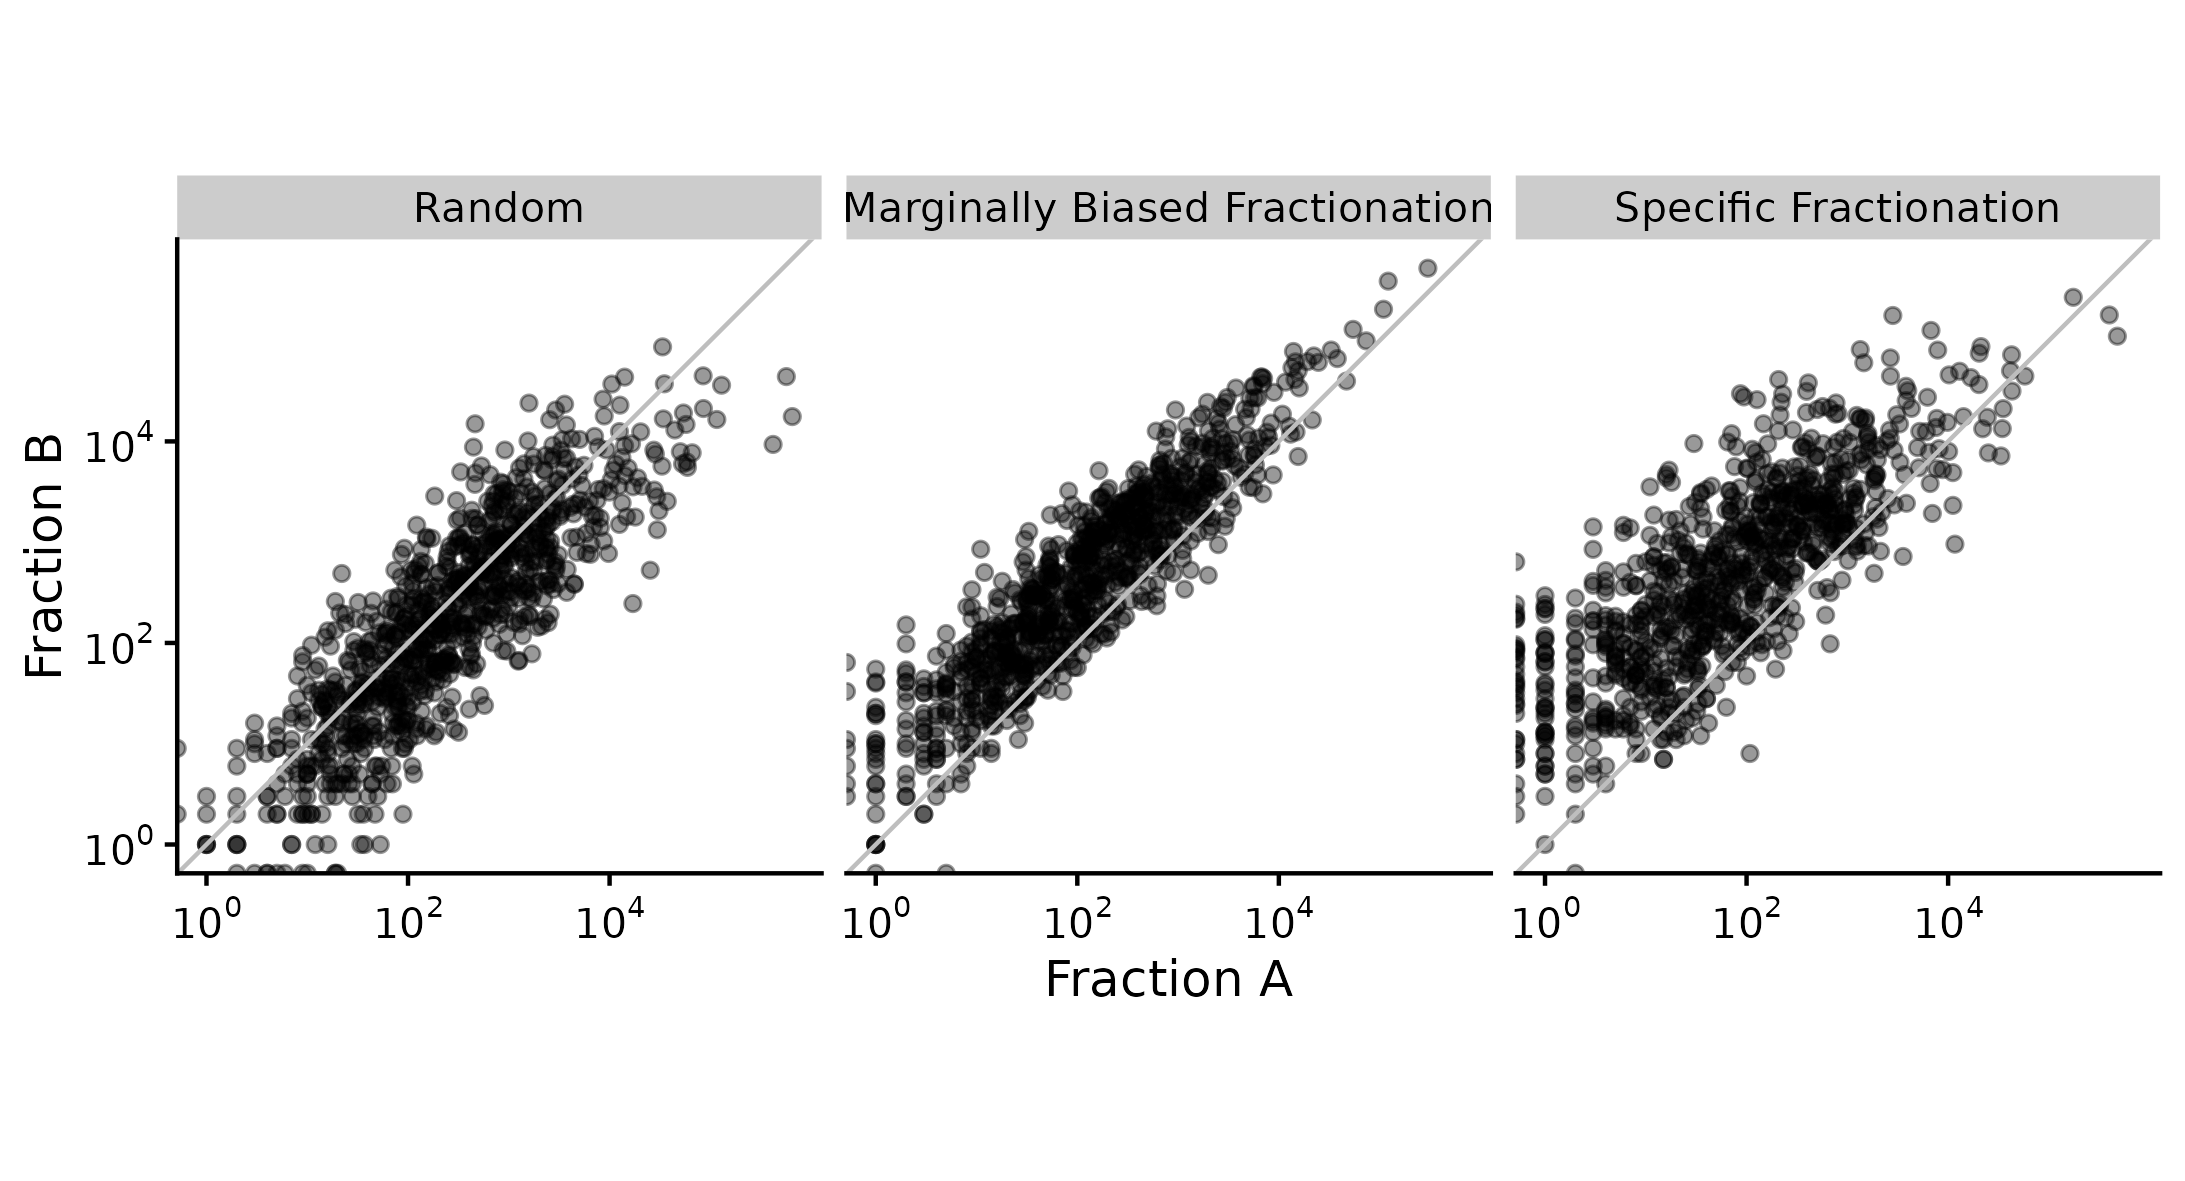
\includegraphics[width=0.8\linewidth]{figures/fractionation_simulated_dataset_summary.png} 

}

\caption[Summary of the simulated test data set.]{\textbf{Overview of the simulated data set used in this study.} Simulated mRNA transcript counts between two fractions in three regimes: all genes are randomly allocated a fraction, most genes have a marginal bias towards fraction B, and the majority of transcripts are in fraction B but transcripts from a specific subset of genes are found in fraction A.} \label{fig:fractionation-simulated-datasets}
\end{figure}

\subsection{Posterior checks using the simulated test data set}

Posterior checks confirm the reliability of the DiffFracSeq model as it correctly recreates the simulated test data set. 
The three replicates of noisy $N^{Tot}$, $N^{A}$ and $N^{B}$ counts from each regime of the simulated data set are used to train the DiffFracSeq model.
1000 samples of all parameters are taken from the posterior distribution after a 1000 iteration burn-in.
The median value of the 1000 samples is used as a summary statistic for all parameters.
$N^{Tot}$, $N^{A}$ and $N^{B}$ counts from the simulated data set are compared to the posterior samples taken from the DiffFracSeq model, Figure \ref{fig:simulated-posterior-check}. 
The counts sampled from the DiffFracSeq model show the model explains the majority of the variation in the counts from the ground truth with $R^2$ values of 0.999 and 0.996 for counts from the two fractions.
Counts from the total sample vary more from the ground truth, $R^2 = 0.792$, likely due to the distribution being explored in linear space, to enable the addition of fractions A and B, rather than log space.

\begin{figure}

{\centering 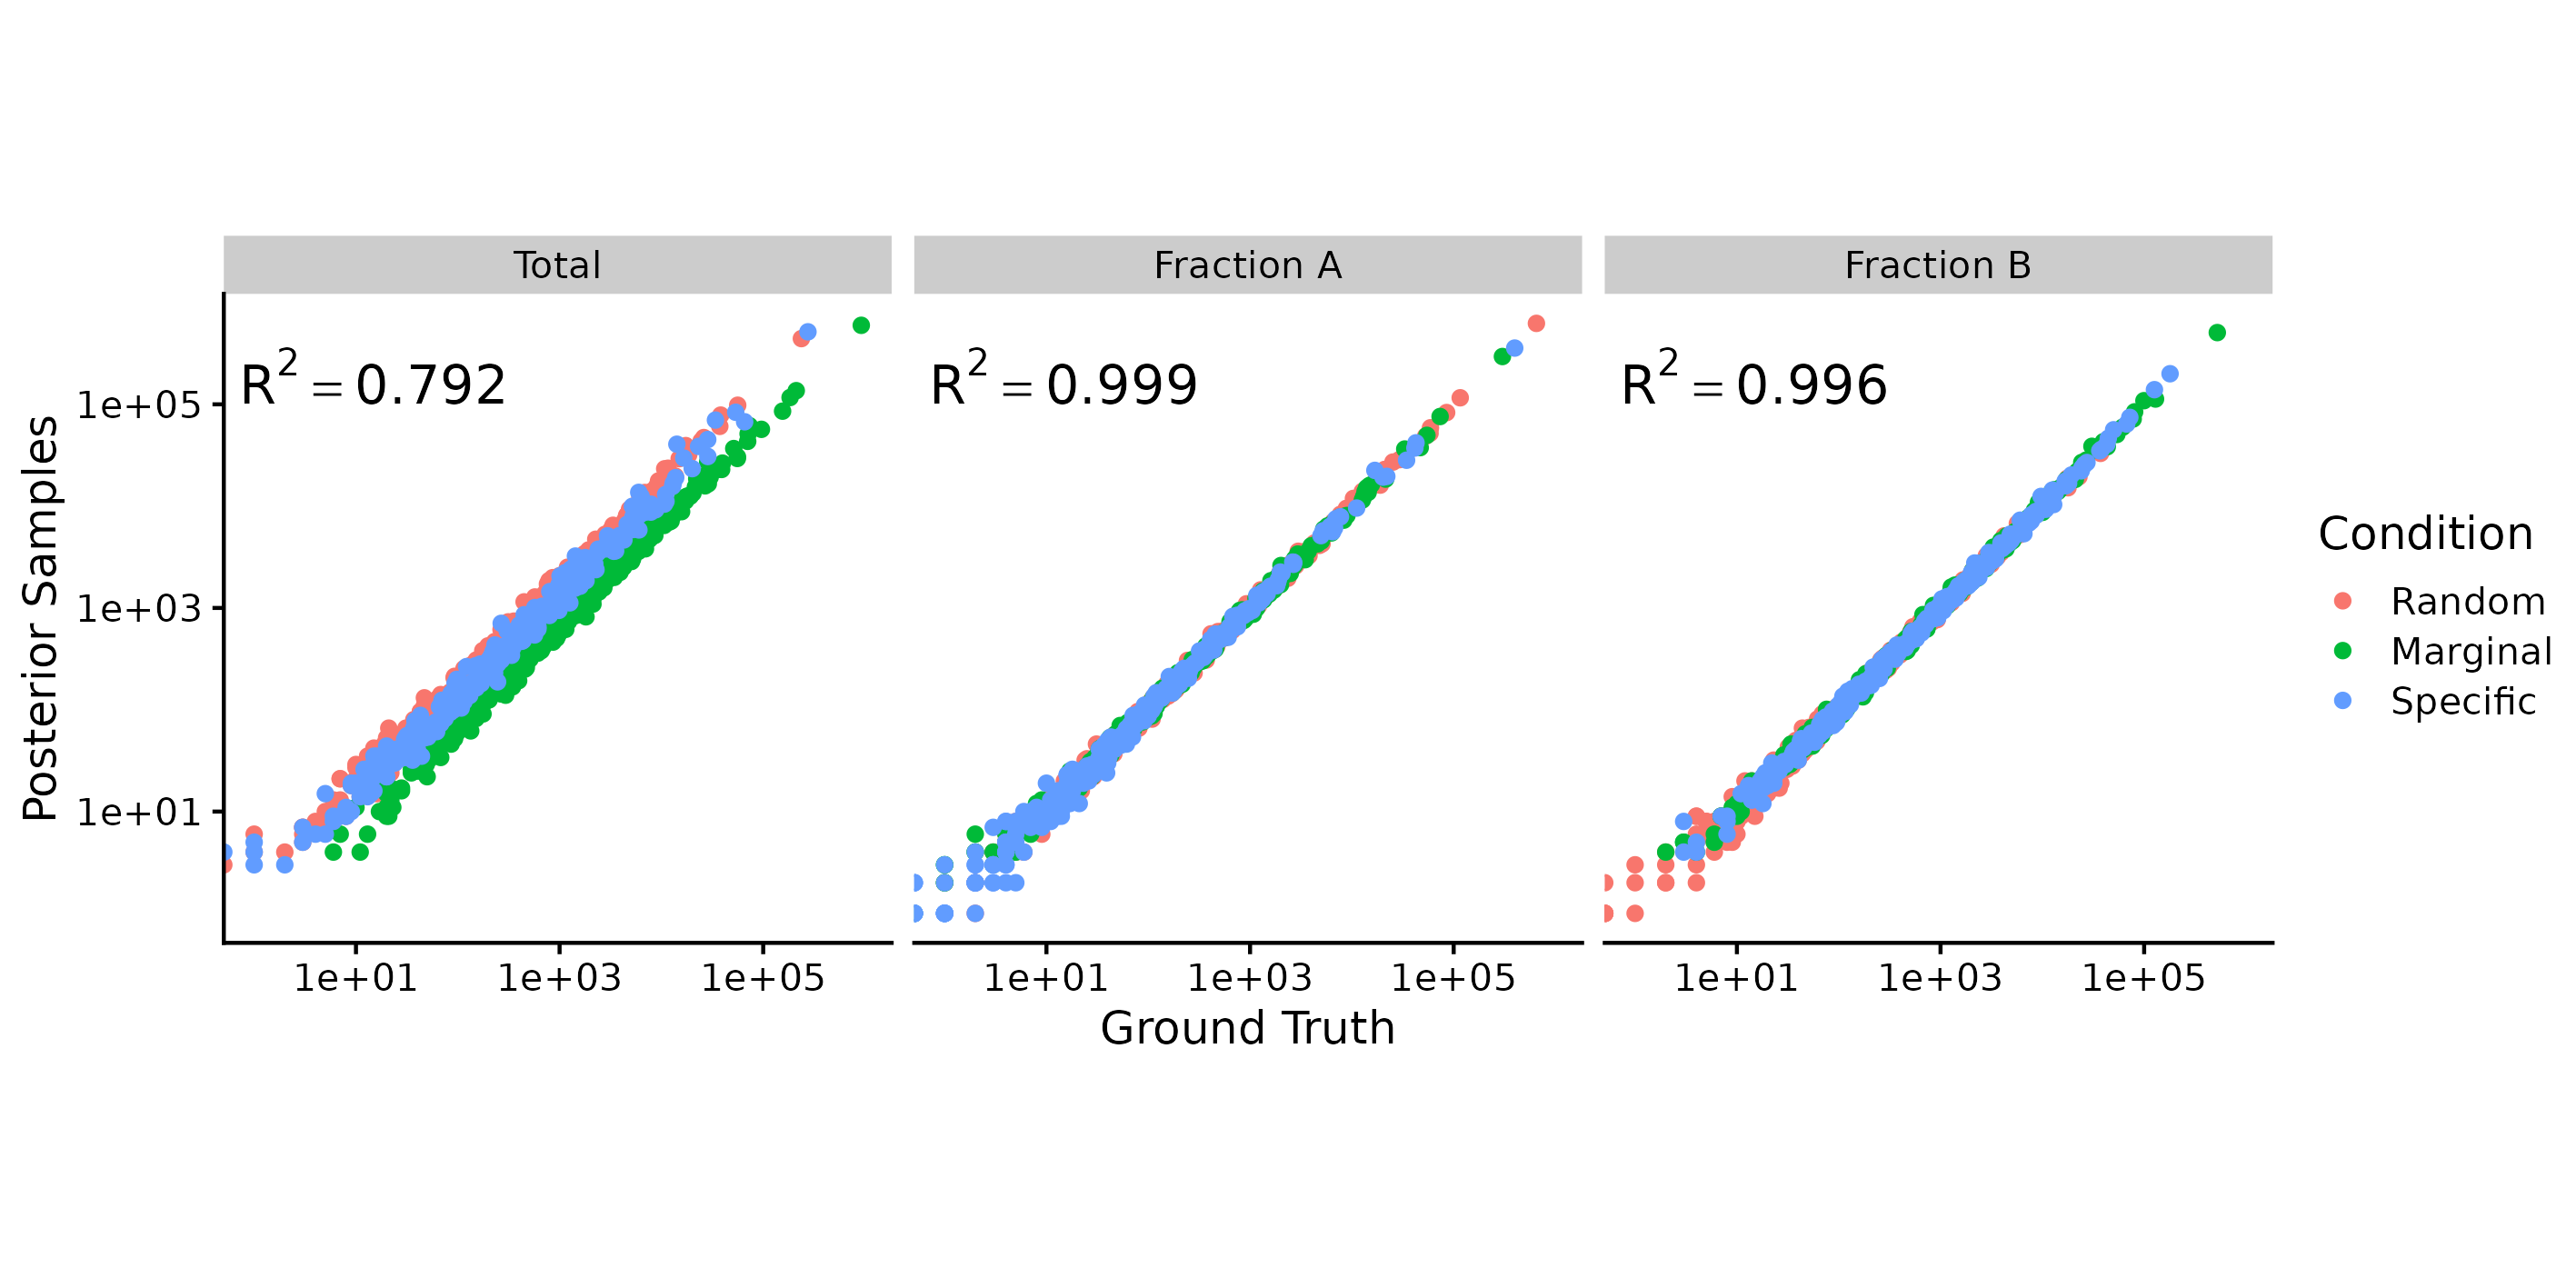
\includegraphics[width=\linewidth]{figures/bayesian_posterior_vs_GT_counts.png} 

}

\caption[DiffFracSeq posterior predictive check]{\textbf{Comparison of noisy transcript counts sampled from DiffFracSeq's posterior distribution to the simulated ground truth.} Noisy transcript counts for all genes in the total sample and both fractions as sampled from DiffFracSeq vs from the simulated ground truth.} \label{fig:simulated-posterior-check}
\end{figure}

\subsection{Detecting differential fractionation using DESeq2}

The detection of differential fractionation with DiffFracSeq is compared to the results of a widely used R package for detecting differential expression using \textit{a priori} normalisation, DESeq2.
To run DESeq2, the counts for a given condition were combined as one matrix with every column holding a different fraction and replicate. 
The design matrix passed to DESeq2 consisted of whether the counts of a gene came from fraction A or fraction B only, \lstinline{design_matrix = ~fraction}.
This method was repeated separately for each of the three conditions, Listing \ref{tab:DESeq2-r-code}.
As well as the determination of normalisation factors, DESeq2 also estimated shrinkage and calculated significance differences using a Wald test following the standard workflow outlined in its documentation. 

\lstdefinelanguage{DESeq}
{morekeywords={data,frame,factor,c,rownames,colnames,DESeqDataSetFromMatrix,DESeq,results},
sensitive=false,
morecomment=[l]#,
morestring=[b]"}

\makeatletter
\renewcommand{\fnum@table}{Listing \thetable}
\makeatother

\begin{table}
\begin{tabular}{c}
\begin{lstlisting}[style=mystyle, language=DESeq]
column_data_simulated <- data.frame(fraction = factor(rep(c("pel",
                                                            "sup"),
                                                          3)),
                                    condition = factor(rep("Random",
                                                           6)))

rownames(column_data_simulated) = colnames(fractionation_count_matrix_simulated)

DESeq2_data_set_simulated_random <- DESeqDataSetFromMatrix(
    countData = fractionation_count_matrix_simulated[,c("random_1_pel", "random_1_sup",
                                                        "random_2_pel", "random_2_sup",
                                                        "random_3_pel", "random_3_sup")], 
    colData = column_data_simulated[1:6,],
    design = ~fraction)

DESeq2_data_set_simulated_random <- DESeq(DESeq2_data_set_simulated_random)


DESeq2_result_simulated_random <- results(DESeq2_data_set_simulated_random)
\end{lstlisting} \\
\end{tabular}
\caption[DESeq2 example R code]{\textbf{Example R code for using DESeq2 to detect differential fractionation in the random regime of the simulated data set.}}
\label{tab:DESeq2-r-code}
\end{table}

\makeatletter
\renewcommand{\fnum@table}{Table \thetable}
\makeatother

\subsection{Detecting differential fractionation with DiffFracSeq and DESeq2 with the simulated ground truth}

The simulated ground truth in gene-wise differential fractionation reveals DiffFracSeq's ability to allow changes in the global transcriptome.
However, DESeq2's normalisation method confounds batch-specific effects with global changes in expression.
The log$_2$ ratio of transcript counts between the two fractions as calculated by DESeq2 and DiffFracSeq were compared to the log$_2$ ratio of noiseless counts in the simulated data set, $\gamma/(1-\gamma)$, Figure \ref{fig:simulated-data-results}A.
The coefficient of variation for the predicted log$_2$ ratio and ground truth is greater than 0.95 for both methods in all regimes. 
Genes considered to be differentially fractionated in faction B over fraction A are highlighted in blue.
For the DiffFracSeq model, a gene is considered to be significantly localised to fraction B if 97.5\% of the $\lambda^{B}$ samples are greater than all of the $\lambda^{A}$ samples for that gene in that regime.
This method provides a suitable summary statistic to compare to DESeq2's frequentist p-value, although DESeq2's results also have an FDR-based multiple-testing correction which is not applied to the DiffFracSeq model p-values.

The disparity between the models is revealed as the difference in the global transcriptome between the two fractions increases across the three regimes in the simulated data sets.
The log$_2$ ratios from DiffFracSeq consistently match the ground truth across all conditions and magnitudes.
However, the log$_2$ ratios from DESeq2 shift below the ground truth for all genes as the fraction transcriptomes change from a balanced 50\%-50\% random regime to an asymmetric 85\%-15\% specific regime.
The shift in log$_2$ ratios across all genes is explained by a divergence in DESeq2's normalisation scale factors in the regimes with asymmetric transcriptomes, Figure \ref{fig:simulated-data-results}B.
In the balanced random regime, DESeq2's normalisation scale factors all follow the same linear relationship with the ground truth scale factor.
For the asymmetric marginal and specific regimes DESeq2's normalisation scale factors for fraction A diverge from the scale factors from fraction B.
Therefore, the absorption of global changes in transcriptome by DESeq2's scale factors limits its ability to detect fractionation.

The shift in DESeq2's log$_2$ ratios is reflected in the detection of significant differential fractionation across all transcript counts.
Across all genes, DESeq2 has a larger false discovery rate (FDR) in the marginal and specific regimes than DiffFracSeq.
In both cases, over 50\% of genes detected to be differentially fractionated by DESeq2 are false positives, but all genes detected by DiffFracSeq are true positives.
Although DESeq2 does have a better FDR in the random regime, 0 vs 0.01, its true positive rate (TPR) is less than DiffFracSeq, 0.78 vs 0.93, Figure \ref{fig:simulated-data-results}C.
This behaviour is replicated over the 60 least abundant genes and the 60 genes with the smallest change between the conditions, Figure \ref{fig:simulated-data-results}D.
Overall, genes determined to be differentially fractionated by DiffFracSeq are more likely to be true positives than those determined by DESeq2.

\begin{figure}

{\centering 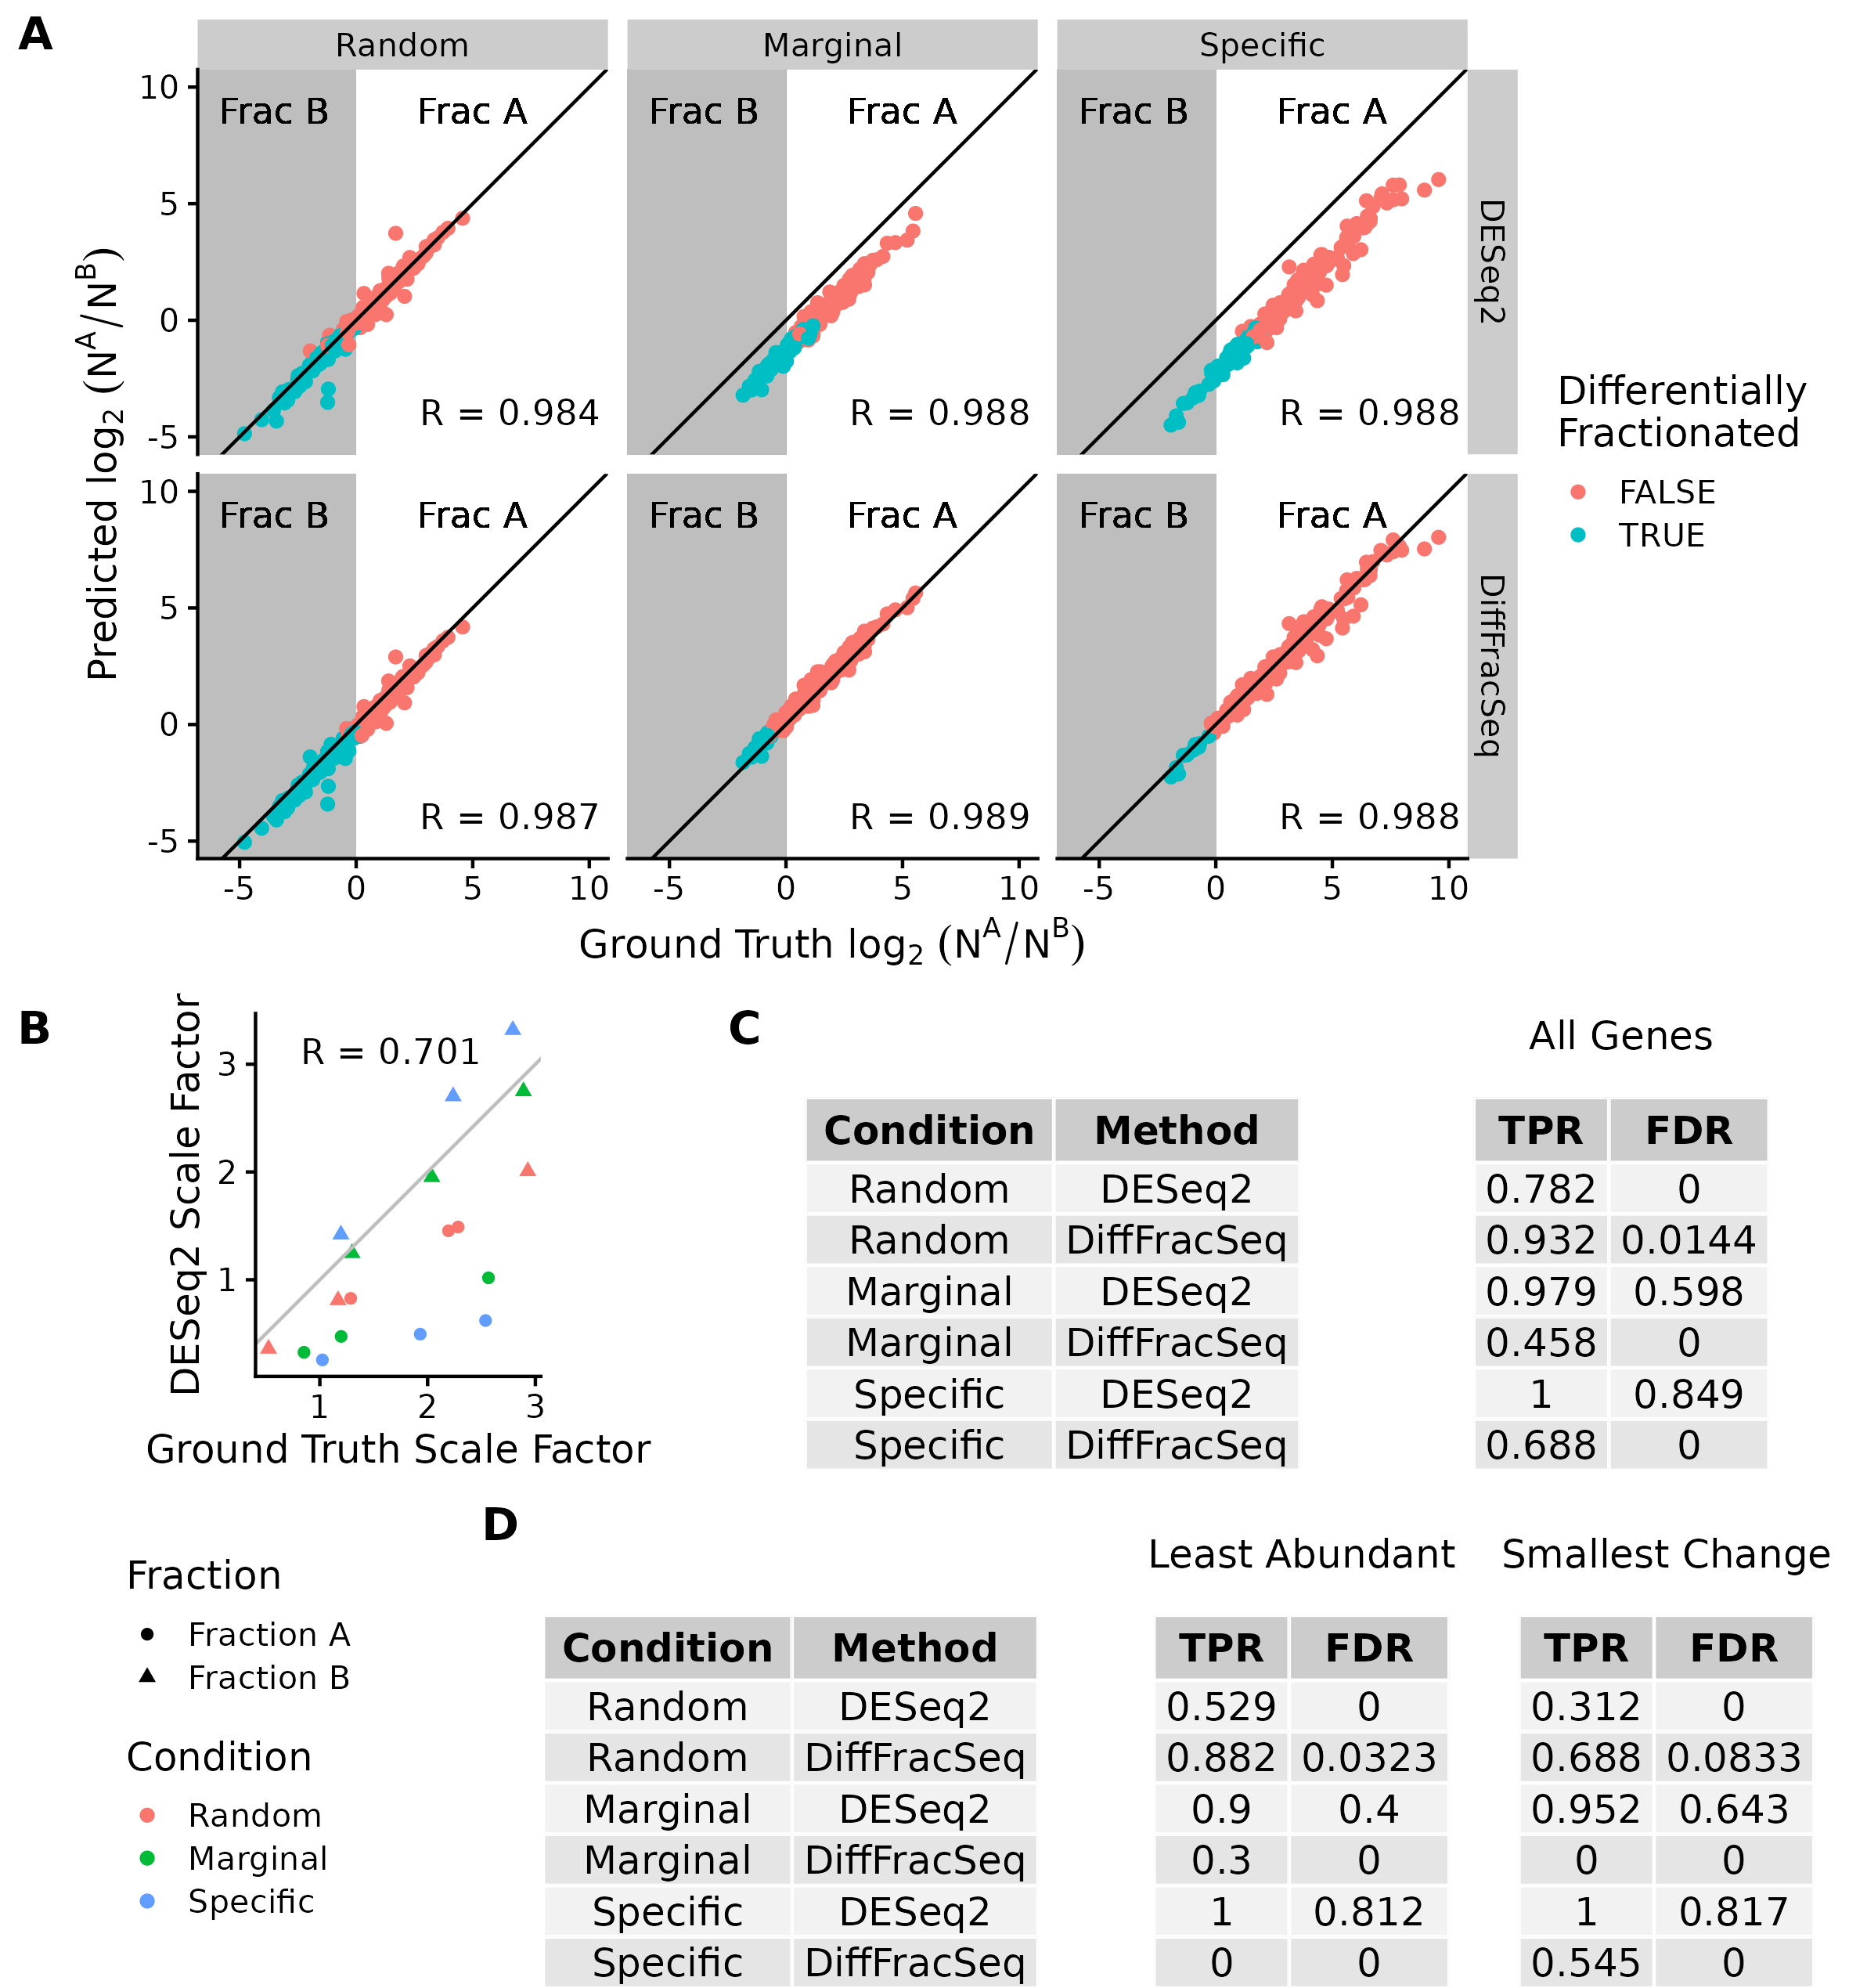
\includegraphics[width=1\linewidth]{figures/DESeq_vs_bayesian_combined.png} 

}

\caption[DiffFracSeq vs DESeq2 performance on the simulated data set.]{\textbf{Comparison of DESeq2 and DiffFracSeq performance a simulated data set.} \textbf{A} Predicted vs ground truth log$_2$ ratio of transcripts in fraction A to fraction B. The first row presents the results determined from DESeq2 and the second row presents the results from DiffFracSeq. The results from the three regimes in the simulated data set are shown across the columns. \textbf{B} Comparison of DESeq2 values of RNA-Seq run specific total read scale factors to the ground truth. \textbf{C} True positive rates (TPR) and false discovery rates (FDR) of the two methods across three regimes for all genes. \textbf{D} Similar to \textbf{C} but across the 60 least abundance genes and the 60 genes with the smallest change between fractions.} \label{fig:simulated-data-results}
\end{figure}

\subsection{Overview of the experimental test data sets}

DiffFracSeq is shown to handle the scale of real experimental data sets by analysing the results of a $\approx16,000$ gene fractionation experiment.
The experimental data set compares the nuclear and cytoplasmic transcriptomes of human cells.
The data set is from the Encyclopedia of DNA Elements (ENCODE) consortium  \parencite{Dunham2012}. 
The data set consists of total, nuclear and cytoplasmic poly(A) RNA transcripts from a human GM12878 lymphoblastoid cell line.
The fractions were separated using centrifugation and include two biological replicates which have a high correlation, Figure \ref{fig:fractionation-datasets}A.
The reads were already aligned to the hg38 human reference genome and counted by the RSEM software \parencite{Li2011} following the standard ENCODE analysis pipeline \parencite{Luo2020}.
It was downloaded from the ENCODE portal with the following identifiers: ENCSR000COR, ENCSR000COQ, ENCSR000CPO.

Finally, DiffFracSeq's ability to detect changes in the fractionation of the transcripts of a gene across conditions is tested using a multi-temperature yeast data set \parencite{Iserman2020}.
This experimental data set is from a paper investigating the transcriptomes of heat-induced stress granules at 30$\degree$C, 40$\degree$C and 42$\degree$C in \textit{Saccharomyces cerevisiae}.
Stress granules were isolated in pellets by 18,000g centrifugation before their transcriptomes were extracted and sequenced.
Samples from the total transcriptome were taken before centrifugation and samples of the unbound transcriptome were taken using the supernatant post-centrifugation.
Two highly correlated biological replicates are available on GEO with accession GSE131176, Figure \ref{fig:fractionation-datasets}B.
The reads were already aligned to the S288C reference genome (release R64-2-1) and counted using the STAR aligner \parencite{Dobin2013}.
The \textit{Saccharomyces} data set also includes a deletion strain in each of the three temperatures, but it is not used here. 

\begin{figure}

{\centering 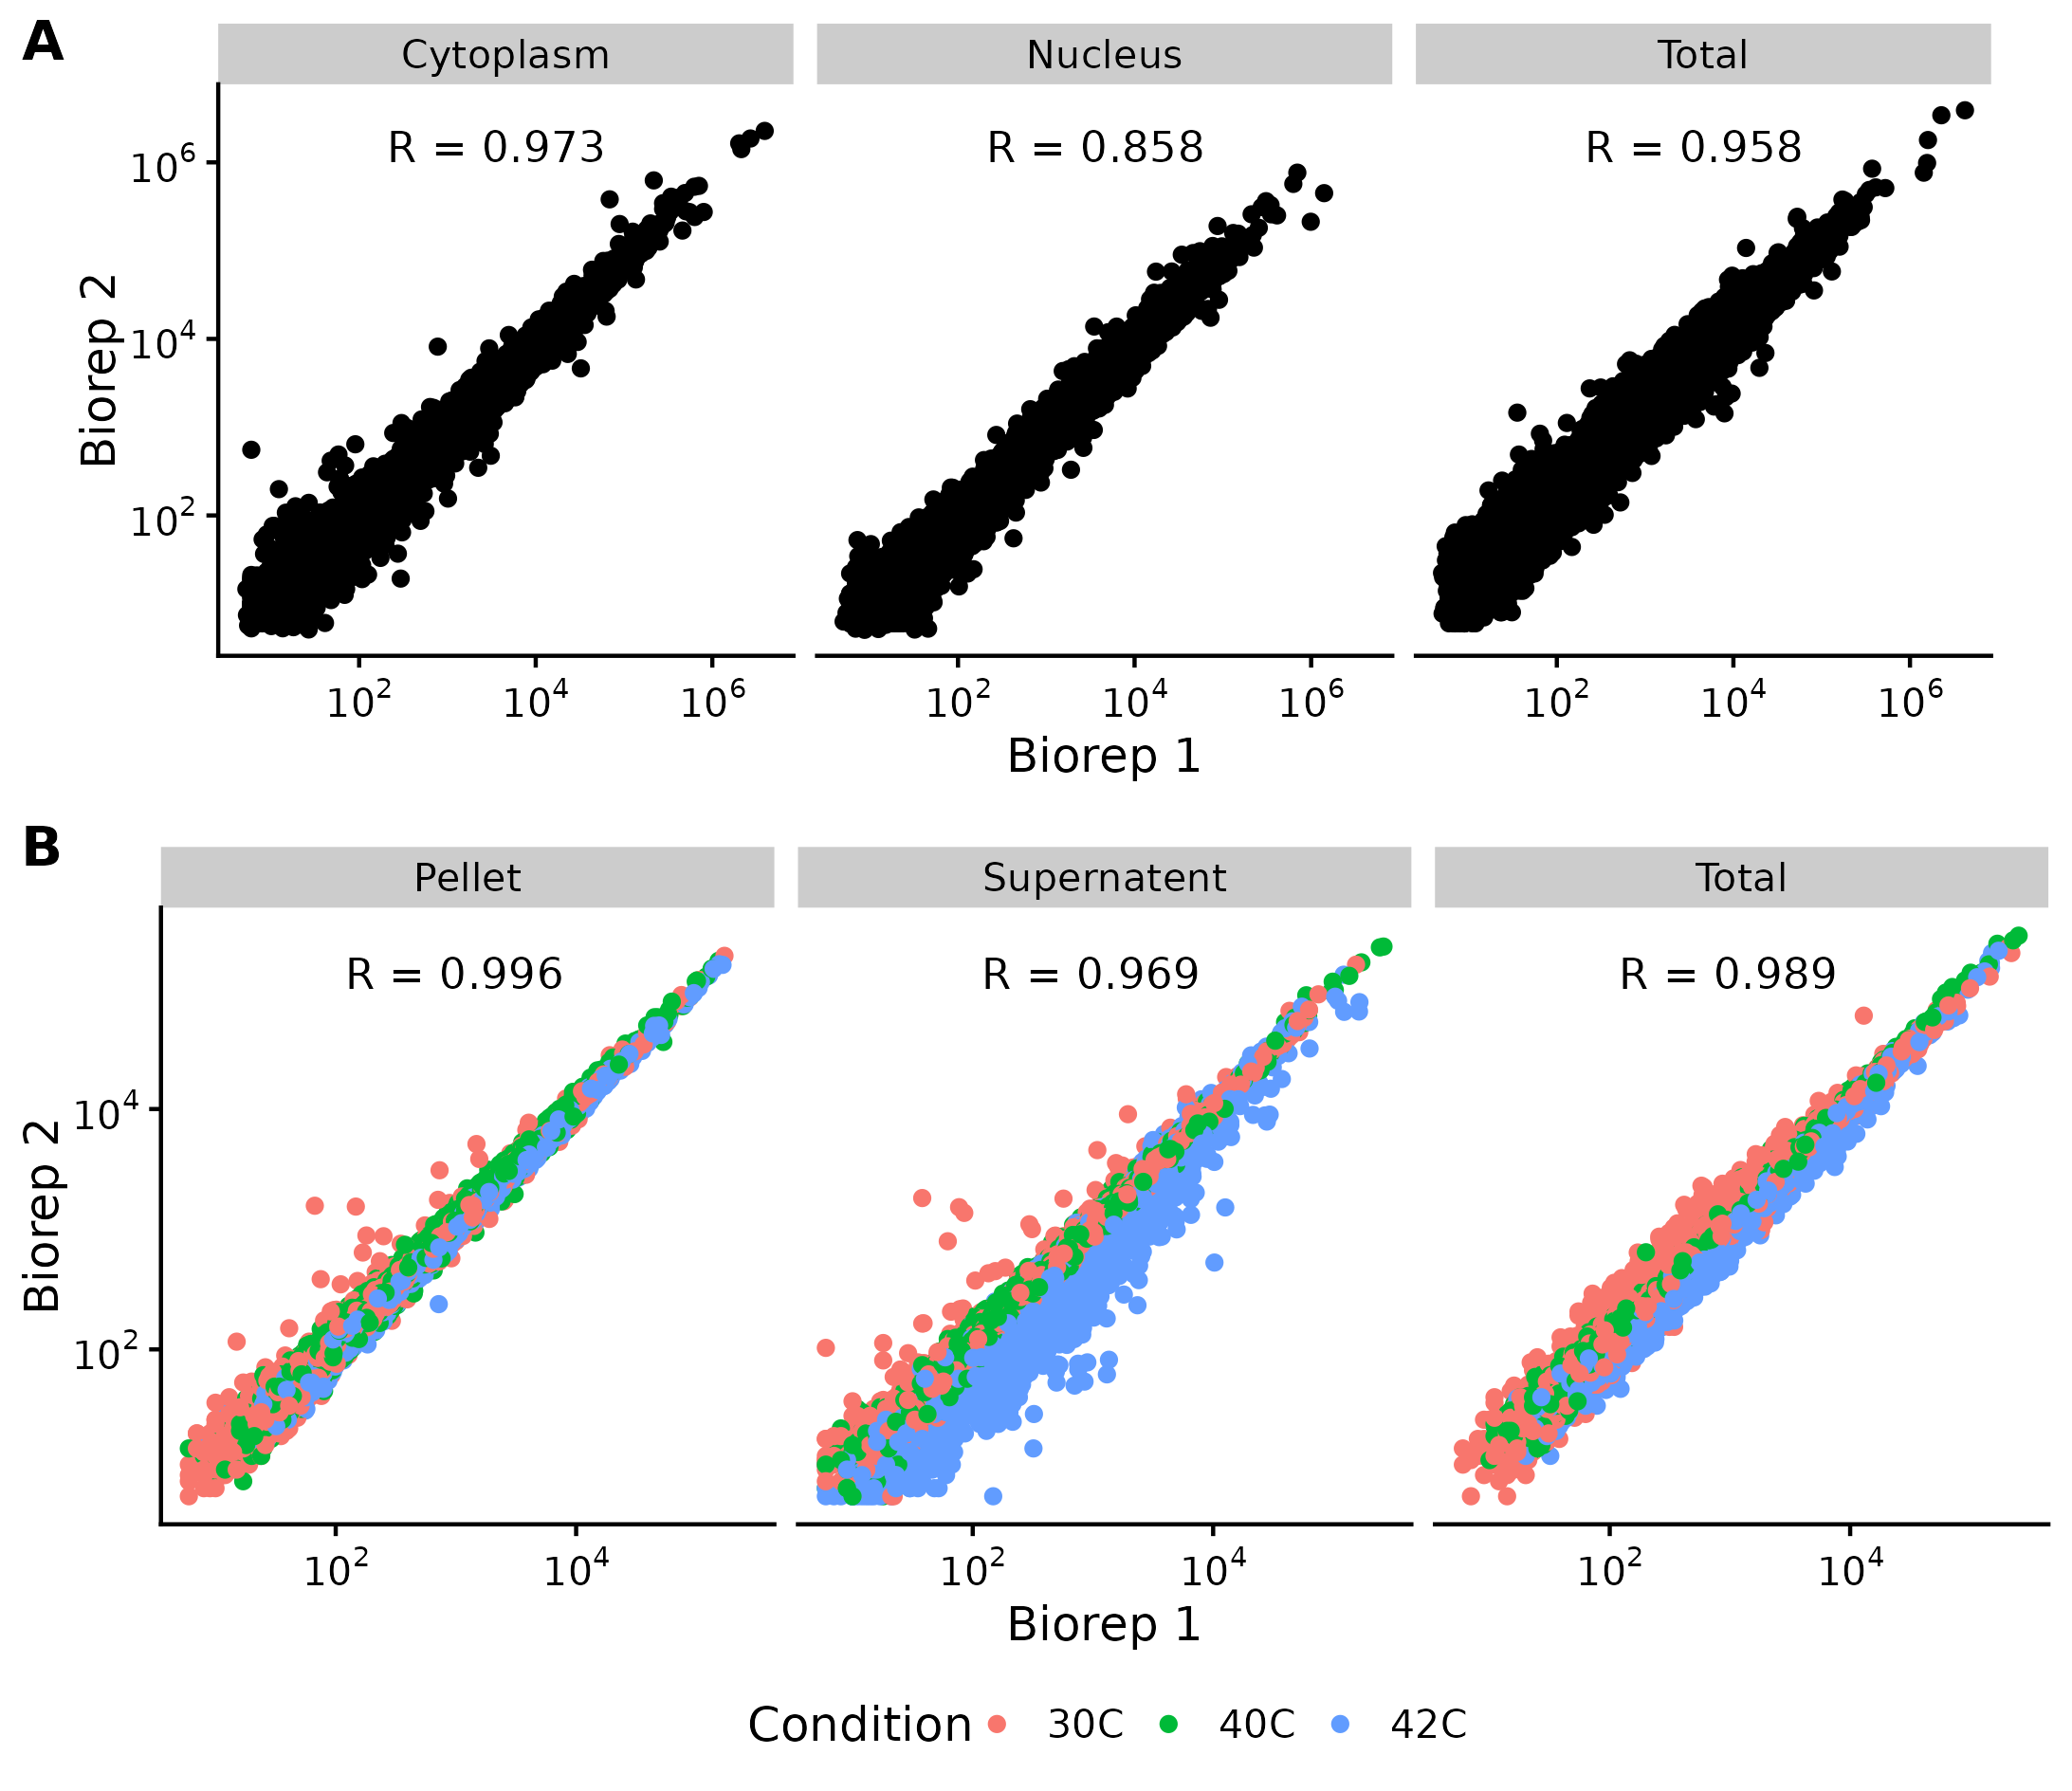
\includegraphics[width=0.95\linewidth]{figures/fractionation_experimental_dataset_summary.png} 

}

\caption[Summary experimental test data sets.]{\textbf{Overview of the two experimental data sets used in this study.} \textbf{(A)} Correlation between two biological replicates of nuclear vs cytoplasmic mRNA transcript counts in a human lymphoblastoid cell line from the ENCODE project \parencite{Dunham2012}. \textbf{(B)} Correlation between two biological replicates of mRNA transcript counts in heat-shock-induced stress granules vs freely floating in \textit{Saccharomyces} cerevisiae cells. The dataset includes three temperature conditions: optimal 30C, mild 40C heat-shock, and extreme 42C heat-shock  \parencite{Iserman2020}.} \label{fig:fractionation-datasets}
\end{figure}

\subsection{Quantifying fractionation in the experimental data sets}

In contrast to DESeq2, DiffFracSeq trained on the ENCODE data set suggests the nuclear transcriptome is more selective and that it predominately consists of ncRNA.
Similar to the results from the simulated data set, the correlation in log$_2$ fraction ratios between the two methods is high, but DiffFracSeq is able to suggest a more asymmetric distribution in total transcript counts between the two fractions, \ref{fig:encode-iserman-data-results}A.
DiffFracSeq determines that over 90\% of poly(A) tailed RNA transcripts are significantly localised to the cytoplasm, compared to 30\% for DESeq2.
Over half of the 234 genes that DiffFracSeq detects as nuclear localised are associated with ncRNA, according to the PANTHER database \parencite{Mi2013}. 
DESeq2 detects almost 20 times more genes as fractionated to the nucleus, 70\% of which are known to be mRNA.

The use of the total transcriptome sample as a quasi-replicate allows DiffFracSeq to detect differential fractionation without any experimental replicates.
The results from training DiffFracSeq using one of the replicates in the ENCODE data set were compared to the results when using both. 
The results between using one and two replicates are correlated, $R = 0.84$ with 185 determined to be differentially expressed using either data set, \ref{fig:encode-iserman-data-results}B.
However, 49 genes are only detected to be significantly localised to the nucleus when using both replicates and 367 additional genes are detected to be significantly localised when using just one replicate.
A similar analysis is not available when using DESeq2 as it requires at least two replicates for each RNA-Seq sample.

DiffFracSeq can detect global changes in the stress granule transcriptome as temperatures increase.
DESeq2 and DiffFracSeq were trained on the Iserman \textit{et al} data set on the yeast stress granule transcriptome at 30$\degree$C, 40$\degree$C and 42$\degree$C. 
DiffFracSeq and DESeq2 have similar correlations in log$_2$ ratio across the temperatures. However, there is a global shift in ratios between the two methods at 30$\degree$C that reduces as the temperature increase to 40$\degree$C and 42$\degree$C, Figure \ref{fig:encode-iserman-data-results}C.
DiffFracSeq detects an increasing number of genes that are differentially fractionated to the stress granule across temperatures with 144, 956, and 2,174 genes selected at 30$\degree$C, 40$\degree$C, and 42$\degree$C respectively.
DESeq2 detects a relatively consistent number of genes as differentially fractionated to the stress granule across temperatures with 1,952, 2,196, and 1,862 genes selected at 30$\degree$C, 40$\degree$C, and 42$\degree$C respectively.

The 40$\degree$C stress granule transcriptome as determined by DiffFracSeq lacks transcripts from genes that are crucial for fundamental cellular processes.
A gene ontology analysis was conducted using PANTHER on genes detected to be differentially fractionated in the pellet at $40\degree$C by DiffFracSeq or by DESeq2.
Genes associated with primary metabolic processes, including those associated with processing organic substances and nitrogen compounds, are significantly underrepresented in the DiffFracSeq subset.
The DESeq2 subset of genes included the same number of genes associated with primary metabolic processes as would be expected if the same number of genes were randomly sampled from the yeast genome.
Instead, the DESeq2 subset was enriched with genes relating to localisation and transmembrane transport. 

\begin{figure}

{\centering 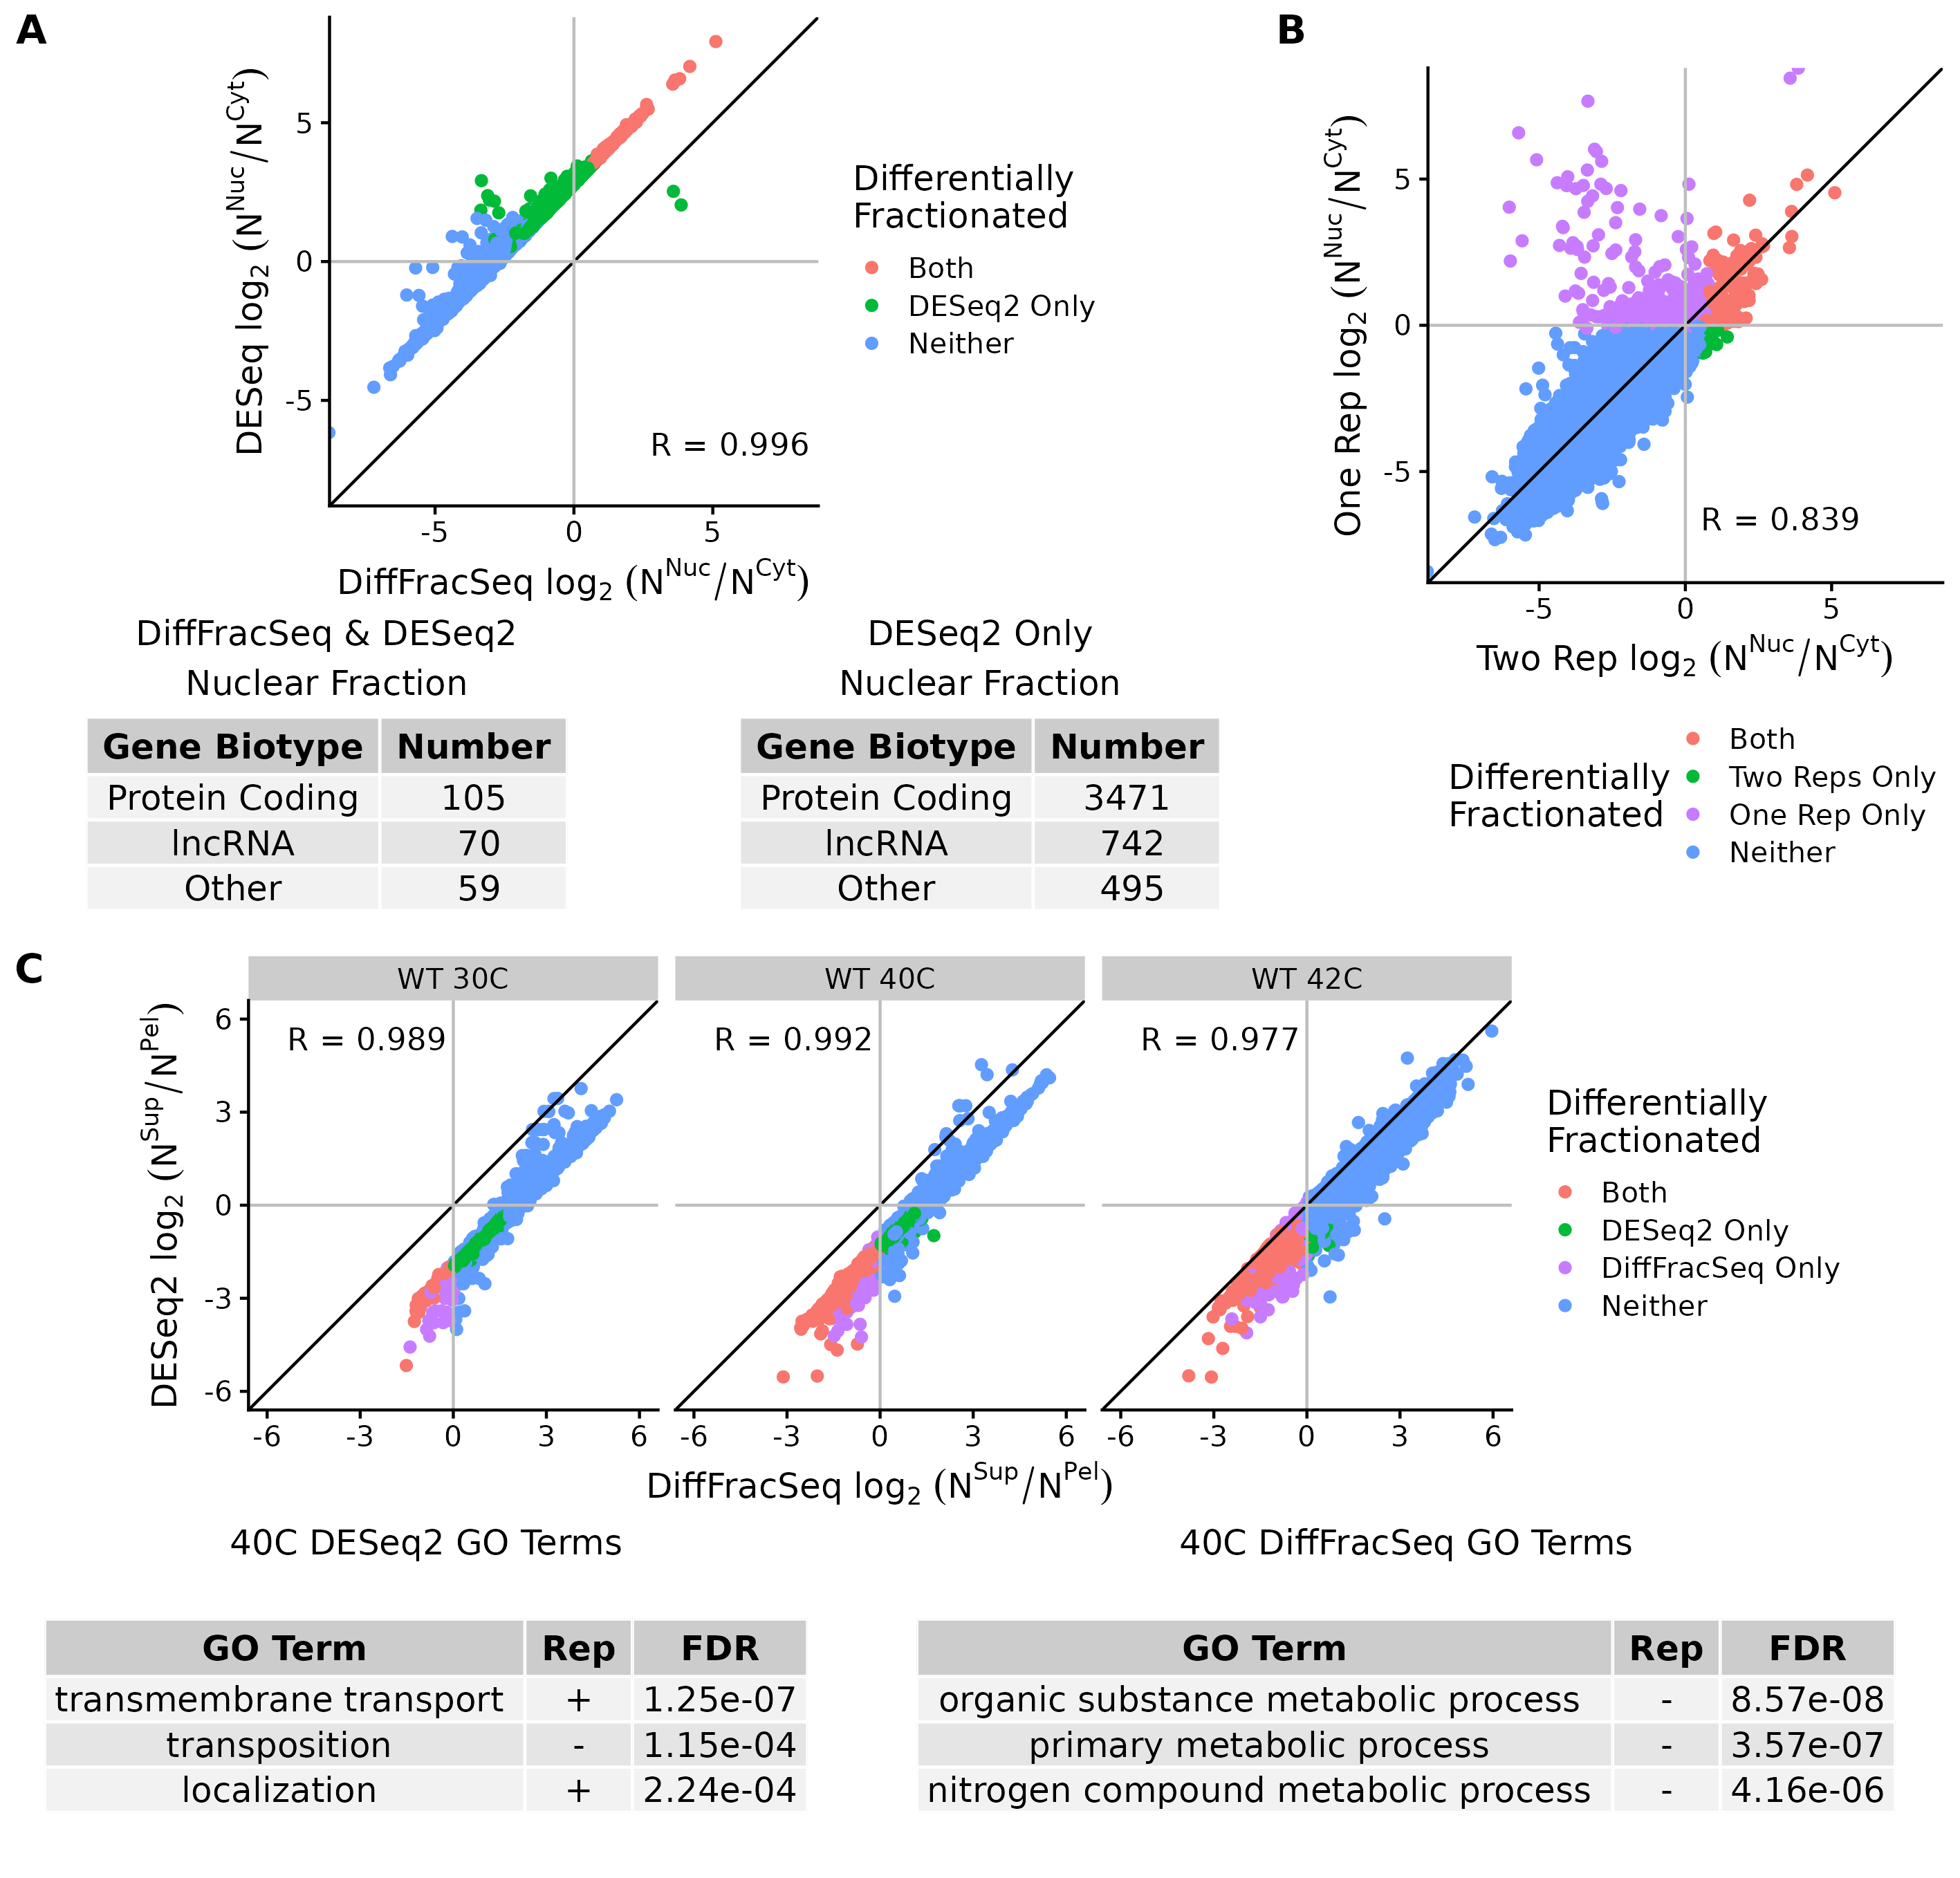
\includegraphics[width=1\linewidth]{figures/DESeq_vs_bayesian_encode_and_iserman_combined.png} 

}

\caption[DiffFracSeq vs DESeq2 performance on the experimental data sets.]{\textbf{Comparison of DESeq2 and DiffFracSeq performance on two experimental data sets.} \textbf{(A)} DESeq2 vs DiffFracSeq predicted log$_2$ ratio of transcripts in the nucleus to the cytoplasm from the ENCODE data set. The colour denotes whether DiffFracSeq or DESeq2 consider the gene to be differentially fractionationed to the nucleus. The two tables show the associated biotype of genes considered differentially fractionated either by both methods or by DESeq2 only, as retrieved from PANTHERdb. \textbf{(B)} DiffFracSeq predicted log$_2$ ratio of transcripts when trained with both or only one of the biological replicates in the ENCODE data set. \textbf{(C)} DESeq2 vs DiffFracSeq predicted log$_2$ ratio of transcripts in the supernatant to the pellet from the Iserman \textit{et al} data set. The wild type samples across three temperature conditions are shown across the columns. The colour denotes whether DiffFracSeq or DESeq2 considers the gene to be differentially fractionationed to the stress granule. The two tables show the top three terms in a gene ontology analysis conducted on genes that are considered differentially fractionated either by DESeq2 only or by DiffFracSeq only in the $40\degree$C condition. The second column of each table denotes whether the GO term is overrepresented ($+$) or underrepresented ($-$) in the gene group.} \label{fig:encode-iserman-data-results}
\end{figure}
\newpage
\subsection{Extending DiffFracSeq to include a generalised linear model on transcript counts}

DiffFracSeq's Bayesian model was extended to determine whether changes in transcript counts across conditions were due to changes in the overall RNA abundance in each fraction or changes in the ratio of RNA abundance between fractions.   
The original model enabled comparisons of transcript counts between fractions of the same sample by accounting for differences in the global transcriptomes of each fraction.
However, the comparison of transcript counts from the same fraction across samples with different conditions, i.e. counts in stress granules across different temperatures, remains unsolved as the counts from each condition are normalised to different quasi-replicates, i.e. total transcript counts prior to centrifugation.
This problem can be addressed by re-introducing the normalising assumption used by DESeq2 and applying it to total transcript counts across conditions.
Assuming the majority of genes have constant transcripts counts in the total transcriptome across all conditions allows for the determination of batch-specific scale factors between samples and conditions.
DiffFracSeq can then detect relative changes in the total expression of a subset of genes.

Decomposing changes in the transcript counts of a fraction across conditions was enabled by introducing a linear model of latent counts, $\lambda^A$, $\lambda^B$, with three terms: $\mu^{Base}$, $\mu^{Con}$, and $\mu^{Frac}$.
$\mu^{Base}$ is shared across all conditions and fractions and represents the base expression of a given gene.
$\mu^{Con}$ is shared across fractions and represents the change in the overall expression of a given gene across conditions.
$\mu^{Frac}$ is unique to fraction B for each condition and represents the change in fractionation of a given gene across conditions.
$\mu^{Base}$ has a broad normal prior to enable the model to correctly determine the range of transcript abundances across a genome.
The prior distributions for $\mu^{Con}$ and $\mu^{Frac}$ are normal distributions with zero mean to encourage the model to set parameters to zero if it believes there are no changes across conditions.
The linear model with normal noise shares the same variance parameter, $\sigma^2$, across all conditions, fractions and genes.
Finally, a hyperparameter, $\alpha$, was added as the mean of the scale factor prior distribution to enable the model to find an appropriate average value for the scale factors given the high variability of this parameter across batches.


\begin{figure}  [p]
     \centering
     \begin{subfigure}[b]{0.4\textwidth}
     \centering
     \tikz{
        % Nodes
        \node[obs]                                   (N-t)   {$N^{Tot}_{grc}$}; %
        \node[obs, above=1 of N-t, xshift=-1.2cm]     (N-s)   {$N^{A}_{grc}$}; %
        \node[obs, right=1 of N-s, xshift=0.4cm]     (N-p)   {$N^{B}_{grc}$}; %
        \node[latent, above=1 of N-s, yshift=0.5cm]  (l-s)   {$\lambda^{A}_{gc}$}; %
        \node[latent, above=1 of N-p, yshift=0.5cm] (l-p)   {$\lambda^{B}_{gc}$}; %
        \node[latent, left=2 of N-t, xshift=0.15cm] (p-t)     {$\phi^{Tot}$}; %
        \node[latent, left=1 of N-s, xshift=0.25cm] (p-s)     {$\phi^{A}$}; %
        \node[latent, right=2 of N-p, xshift=0cm] (p-p)     {$\phi^{B}$}; %
        \node[latent, below=1 of N-t] (a-t)     {$a^{Tot}_{cr}$}; %
        \node[latent, left=1 of a-t, xshift=0.3cm] (a-s)     {$a^{A}_{cr}$}; %
        \node[latent, right=1 of a-t, xshift=-0.2cm] (a-p)     {$a^{B}_{cr}$}; %
        \node[latent, below=3 of N-t, yshift=-0.4cm] (alpha-p)     {$\alpha$}; %
        \node[latent, above=2 of N-t, yshift=0.3cm] (mu-con)     {$\mu^{Con}_{gc}$}; %
        \node[latent, above=5 of N-t, yshift=-0.2cm, xshift=-0.05cm] (mu-base)     {$\mu^{Base}_{g}$}; %
        \node[latent, right=1 of l-p, xshift=-0.3cm] (mu-frac)     {$\mu^{Frac}_{gc}$}; %
        \node[latent, above=3 of mu-con, yshift=0.5cm] (sigma)     {$\sigma^2$}; %
        
        
        % Connections
        \edge {a-t} {N-t} ; %
        \edge {a-s} {N-s} ; %
        \edge {a-p} {N-p} ; %
        \edge {p-t} {N-t} ; %
        \edge {p-s} {N-s} ; %
        \edge {p-p} {N-p} ; %
        \edge {l-s} {N-t, N-s} ; %
        \edge {l-p} {N-t, N-p} ; %
        \edge {alpha-p} {a-p, a-s} ; %
        \edge {sigma} {l-s, l-p} ; %
        \edge {mu-base} {l-s, l-p} ; %
        \edge {mu-con} {l-s, l-p} ; %
        \edge {mu-frac} {l-p} ; %
        
        % plate
        \plate {rep} {(N-t)(N-p)(N-s) %
                      (a-t)(a-p)(a-s)} {$Rep$}
        \plate {gene} {(l-p)(l-s) %
                       (N-t)(N-p)(N-s) %
                       (mu-base)(mu-con)(mu-frac)} {$Gene$}
        \plate {con} {(N-t)(N-p)(N-s) %
                      (l-p)(l-s) %
                      (rep)%
                      (mu-con)(mu-frac)} {$Con$}
    }
    \end{subfigure}
     \hfill
     \begin{subfigure}[b]{0.5\textwidth}
     \centering
     \begin{align*}
        N^{Tot}_{grc} & \sim  negbin(a^{Tot}_{cr}(e^{\lambda^{A}_{gc}} + e^{\lambda^{B}_{gc}}), \phi^{Tot})\\
        N^{B}_{grc} & \sim  negbin(e^{a^{B}_{cr}+\lambda^{B}_{gc}}, \phi^{B})\\
        N^{A}_{grc} & \sim  negbin(e^{a^{A}_{cr}+\lambda^{A}_{gc}}, \phi^{A})\\
        \\
        \lambda^{A}_{gc} &\sim normal(\mu^{Base}_{g} + \mu^{Con}_{gc}, \sigma^2)\\
        \lambda^{B}_{gc} &\sim normal(\mu^{Base}_{g} + \mu^{Con}_{gc} + \mu^{Frac}_{gc}, \sigma^2)\\
        \mu^{Base}_{g} &\sim normal(7,2) \\
        \mu^{Con}_{gc} &\sim normal(0,1) \\
        \mu^{Frac}_{gc} &\sim normal(0,1) \\
        \sigma^2&\sim normal(2,1)\\
        \\
        \phi^{Tot}, \phi^{A}, \phi^{B}&\sim normal(100,10)\\
        a^{A}_{cr}, a^{B}_{cr}&\sim normal(\alpha, 0.1)\\
        \alpha&\sim normal(0, 0.5)
    \end{align*}
     \vspace{0.2cm}
     \end{subfigure}
     \caption[Graphical representation of the DiffFracSeq model with conditions.]{\textbf{Plate diagram summarising the complete Bayesian hierarchical model behind DiffFracSeq.} A generalised linear model of transcript counts across conditions was introduced by adding linear terms, $\mu^{Base}_{g}$, $\mu^{Con}_{gc}$, and $\mu^{Frac}_{gc}$, to the means of the two latent count variables, $\lambda^{A}_{gc}$ and $\lambda^{B}_{gc}$.}
     \label{fig:DiffFracQuant-con-plate-diagram}
\end{figure}

\subsection{Detecting relative changes in fractionation and expression across conditions}

In response to heat-shock, DiffFracSeq determines an increase in transcripts localised to stress granules and a global reduction in expression.
Over 1/5 of genes have a significant increase in the fraction of transcripts found in stress granules over the change from $30\degree$C to $40\degree$C.
Comparing $30\degree$C to $42\degree$C, even more genes are detected to have an increase in fractionation to stress granules, 2421 genes compared to 1407 genes at $40\degree$C.
As temperature increases from $30\degree$C to $40\degree$C DiffFracSeq detects 2373 genes in the yeast genome as significantly underexpressed, i.e. over 97.5\% of $\mu^{Con}_{40\degree C}$ samples are significantly lower than all $\mu^{Con}_{30\degree C}$ samples for a particular gene.
DiffFracSeq detects only 1945 genes as underexpressed for the transition from $30\degree$C to $42\degree$C.
However, as DiffFracSeq is detecting nearly 1/3 of the yeast genome as differentially expressed across conditions the normalising assumption is likely invalid and conclusions about changes in total expression are unreliable.

DiffFracSeq uncovers general behaviours in genes in response to heat shock.
Overall, there is a negative correlation between genes predicted to have an increase in overall expression and genes that change to be more concentrated in the supernatant, {-0.539}, -0.557, and -0.646.
Four categories of behaviour in response to heat stress can be detected by DiffFracQuant: increase in total expression and increase in localisation to the stress granule, decrease in total expression and decrease in localisation to the stress granule, increase in expression and decrease in localisation, and decrease in expression and increase in localisation.
For example, 191 genes at $42\degree$C  and 72 genes at $40\degree$C  are detected to increase in expression and  fractionation to stress granules as temperature increases from $30\degree$C \ref{fig:diff-exp-temp}.


\begin{figure}

{\centering 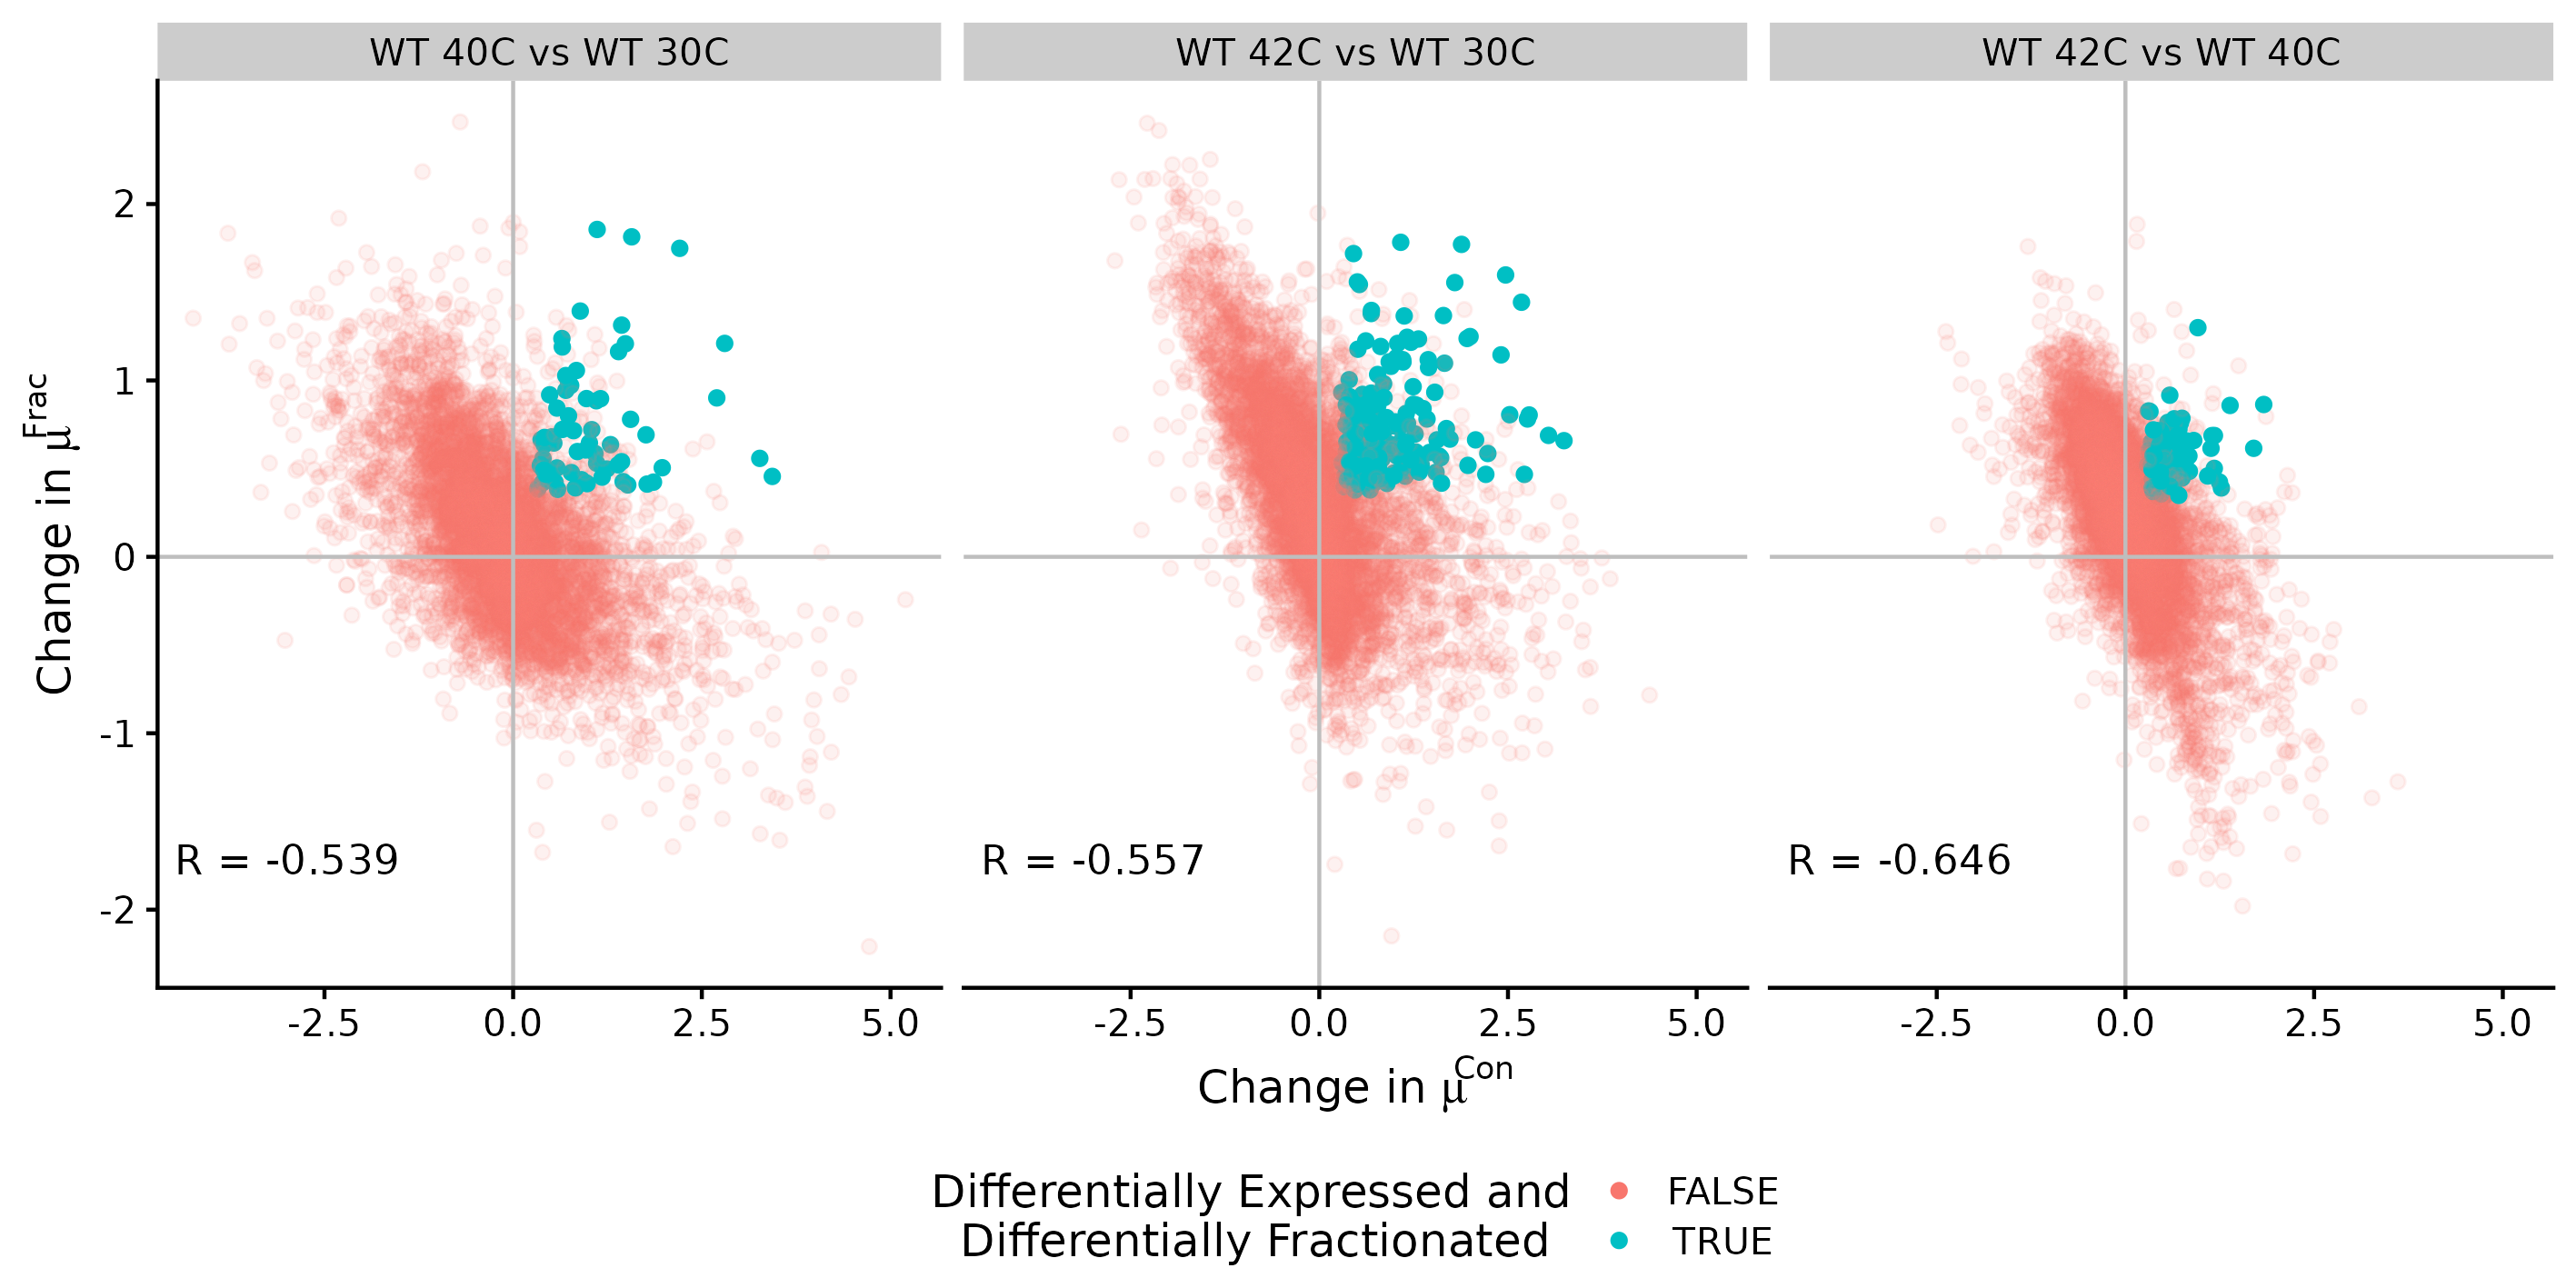
\includegraphics[width=1\linewidth]{figures/DESeq_vs_bayesian_multi_temp_iserman_combined.png} 

}

\caption[Detection of differential expression and fractionation across temperatures.]{\textbf{Detection of differential fractionation and differential expression across the Iserman data set.} Changes in $log_2$ fold expression, $\mu^{Con}$, vs changes in $log_2$ fold ratio between fractions, $\mu^{Frac}$, between all pairs of the three conditions.
Genes in the top left quadrant are overexpressed at the higher temperature and more localised to the stress granule. Genes in the bottom right quadrant are underexpressed in the higher temperature and are more localised to the cytoplasm. Genes that DiffFracSeq detects as differentially fractionated and differentially expressed across the pair of conditions are highlighted in blue.} \label{fig:diff-exp-temp}
\end{figure}

\section{Conclusion}

\begin{figure} 
     \centering
     \begin{subfigure}[b]{0.53\textwidth}
     \centering
     \tikz{
        % Nodes
        \node[obs]                     (N-t)   {$N^{Tot}_{grc}$}; %
        \node[obs, right=1 of N-t, xshift = 0.6cm]     (N-f)   {$N^{Frac}_{grcf}$}; %
        \node[latent, above=1 of N-f, xshift = -1.3cm]  (l-f)   {$\lambda^{Frac}_{gcf}$}; %%
        \node[latent, below=4 of N-t, yshift = -0.15cm]   (p-t)     {$\phi^{Tot}$}; %
        \node[latent, right=2 of N-f, xshift = -0.40cm]  (p-f)     {$\phi^{Frac}_f$}; %
        \node[latent, below=2 of N-t, xshift = -1.5cm, yshift = 0.2cm]  (a-t)     {$a^{Tot}_{cr}$}; %
        \node[latent, below=1 of N-f, xshift = -1.2cm]  (a-f)     {$a^{Frac}_{crf}$}; %
        \node[latent, below=1 of a-f, yshift = -1.2cm]  (alpha)     {$\alpha$}; %
        \node[latent, right=1 of l-f, xshift = 0.5cm]  (mu-frac)     {$\mu^{Frac}_{gcf}$}; %
        \node[latent, left=1 of l-f]  (mu-con)     {$\mu^{Con}_{gc}$}; %
        \node[latent, left=1 of l-f, yshift = 1.5cm]  (mu-base)     {$\mu^{Base}_{g}$}; %
        \node[latent, above=2 of l-f, yshift = -0cm]  (sigma)     {$\sigma^2$}; %
        
        
        % Connections
        \edge {a-t} {N-t} ; %
        \edge {a-f} {N-f} ; %
        \edge {p-t} {N-t} ; %
       \edge {p-f} {N-f} ; %
       \edge {l-f} {N-t, N-f} ; %
        \edge {alpha} {a-f} ; %
        \edge {sigma} {l-f} ; %
        \edge {mu-frac} {l-f} ; %
        \edge {mu-con} {l-f} ; %
        \edge {mu-base} {l-f} ; %
        
        % plate
        \plate {frac} {(N-f)(a-f)(p-f)(l-f)(mu-frac)} {$Frac$}
        \plate {rep} {(N-t)(N-f)(a-t)(a-f)} {$Rep$}
        \plate {gene} {(l-f)(N-t)(N-f)(mu-con)(mu-frac)(mu-base)} {$Gene$}
        \plate {con} {(N-t)(N-f)(l-f)(rep)(mu-frac)(mu-con)} {$Con$}
    }
     \end{subfigure}
     \caption[Graphical representation of the multi-fraction DiffFracSeq Model.]{\textbf{Plate diagram summarising an improved multi-fraction model for DiffFracSeq.} The next iteration of the Bayesian hierarchical model behind DiffFracSeq will enable the normalisation and detection of differential fractionation in RNA-Seq experiments with more than two sub-fractions.}
     \label{fig:DiffFracQuant-future-plate-diagram}
\end{figure}

This chapter introduced DiffFracSeq as a novel Bayesian model for analysing RNA-Seq data and, to our knowledge, the only statistical model specifically designed to detect differential fractionation.
The inclusion of pre-fractionation counts as a quasi-replicate to help normalise sub-fraction counts enables the Bayesian model to accurately determine batch-specific scale factors.
The ability of the model to perform even with a single replicate data set and to extract changes in total transcript abundance as well as relative fractions from data sets with multiple conditions means it is a versatile tool in exploring fractionation data sets.

DiffFracSeq's has been shown to outperform DESeq2 in detecting differential fractionation using a simulated data set.
DESeq2's inflated false positive rate is revealed when fractions contain global changes in their transcriptomes.
Even in the 50\%-50\% random regime, when DESeq2's normalisation method successfully accounts for the batch-specific scale factors, DiffFracQuant has a better true positive rate when detecting significant differential fractionation than DESeq2.
This behaviour is repeated across genes with the lowest overall expression and the smallest effect sizes.

DiffFracSeq can determine asymmetric transcript abundances between fractions at scale with the human nuclear-cytoplasmic data set.
Of the $\approx16,000$ uniquely mapped genes, DiffFracSeq only determined 234 genes as having transcripts localised to the nucleus compared to 4708 genes detected by DESeq2.
A recent study by Zaghlool \textit{et al} also analysed the GM12878 cell line, together with three other human cell lines, and similarly determined ~4500 transcripts that are localised to the nucleus using DESeq2, see \parencite{Zaghlool2021} Supplementary Figure 2. 
However, DiffFracSeq's result correlates with the original ENCODE analysis that placed the majority of protein coding transcripts in the cytoplasm without using DESeq2, \parencite{Djebali2012} Figure 3.

DiffFracSeq can determine relative changes in fractionation across conditions in a yeast stress granule data set.
Gene ontology analysis of the heat stress granule transcriptome according to DiffFracSeq shows it lacks key transcripts associated with key metabolic processes.
However, the same analysis using the DESeq2 transcriptome shows enrichment for transmembrane proteins in contradiction to other stress granule studies \parencite{Unworth2010, Khong2017}.
As temperature increases, DiffFracSeq detects more genes as differentially fractionated to the stress granule, but DESeq2 does not have a clear pattern.
DiffFracSeq also detects a correlation between genes that are overexpressed under stressed conditions and increase the fraction of their transcripts in the cytoplasm.
However, further exploration of changes in total expression is limited by the breaking of the underlying normalising assumption used to compare expression across conditions.

DiffFracSeq can only determine relative changes in RNA abundance in each fraction and cannot estimate overall changes in total RNA abundance per cell.
The model can be enhanced to allow normalisation using external RNA spike-ins so that changes in total RNA abundance per cell can be measured across conditions.
The model behind DiffFracSeq can be further expanded by modelling counts from more than two fractions, Figure \ref{fig:DiffFracQuant-future-plate-diagram}.
The linear sum of sub-fraction counts can theoretically be extended to include any number of sub-samples $N^{Tot} = \displaystyle\sum_i N^{i}$.
Enabling more fractions to be normalised could unlock more use cases for the software as it could also be used to characterise libraries of constructs by comparing fractions from cell sorting assays.
Entire libraries of synthetic constructs can be characterised by sorting pools of constructs by some desired characteristic, for example high protein fluorescence, which are subsequently sequenced \parencite{Sharon2012}.
Alternatively, the linear model predicting latent transcript counts could be improved by letting users define their own design matrices.
The latent count linear model is fixed to determine separate coefficients for each condition, but users may be interested in exploring interactions between conditions.
For example, the Iserman \textit{et al} data set also includes stress granule samples from a mutant strain across the three temperatures which could be directly compared to the wild type. 
This assumption enabled DiffFracSeq to detect differential expression and fractionation across conditions, but this functionality is not applicable in many cases.

The software containing the two-fraction model is available to download from GitHub, \href{https://github.com/DimmestP/DiffFracSeq}{github.com/DimmestP/ DiffFracSeq}, and has been shown to be successful at investigating localisation across organisms and subcellular fractions.
DiffFracSeq has the functionality to improve the quality of experiments across biology from the uncovering of novel regulatory mechanisms in fundamental cell biology to the characterisation of constructs libraries in synthetic biology.

\end{document}